%% Capitol 3
% \part{Programació de perifèrics I}
% \label{part:programacio}

En aquest capítol s'aniran introduint i explicant els perifèrics mes habituals que trobem en els microcontroladors actuals. Cada capítol constarà d'una petita introducció al perifèric en qüestió i un petit exemple amb el codi corresponent i els comentaris adients.

\begin{remark}
El tipus de codi que es veurà als exemples es coneix com {\em Baremetal} que vol dir que no es fa servir cap Sistema Operatiu, que es veurà a la \fullref{part:freertos}. Aquests sistemes es basen en les inicialitzacions necessàries i un bucle sense fi al {\bf main()}\index{main()} on es realitzen les operacions desitjades. S'acostuma a usar aquest mètode en aplicacions senzilles o en aplicacions que corren en microcontroladors poc potents o sense prou memòria com per executar còmodament un \gls{RTOS}.
\end{remark}

\chapter{Consola de Debug}
\label{sub:console}
Un de les principals diferències quan treballem amb sistemes encastats és que no tenim una consola on executem el nostre binari i podem veure quins resultats ha obtingut.

Una millora d'ARM respecte arquitectures anteriors va ser la d'incorporar ja fa temps un mecanisme de debug, a través d'un pin d'output anomenat {\em SWO} que permet enviar dades cap a una consola al nostre PC de desenvolupament.

Aquest pin {\em SWO} forma part del sistema de Debug dels Cortex anomenat ITM ({\em Instrumentation Trace Macrocell}) \cite{ITM}. Això vol dir que la majoria de microcontroladors basats en Cortex que ens trobem, siguin del fabricant que sigui portaran aquesta funcionalitat.\footnote{La majoria de Cortex-M0+ no porten aquest perifèric.}

Per poder fer servir aquesta funcionalitat, cal primer configurar el pin SWO per a que funcioni com a tal (es pot fer servir també com un \gls{GPIO} normal). Tot seguit es configura el dispositiu de trace i el mòdul ITM d'aquest. La configuració es fa a la funció {\bf setupSWOForPrint()}\index{setupSWOForPrint()}.

Un cop configurat el mòdul ITM, la funció {\bf ITM\_SendChar()}\index{ITM{\_}SendChar()} permet enviar caràcter a caràcter el que vulguem presentar a la consola a l'altre costat.

En el cas de Simplicity, els caràcters rebuts es presenten directament a la consola de la part d'abaix del \gls{IDE} (Figura~\ref{fig:ITM}).

\begin{figure}
 \centering
 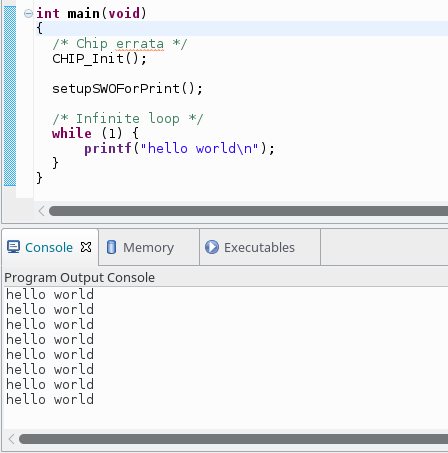
\includegraphics[width=0.85\textwidth, keepaspectratio]{imatges/ITM_Debug.png}
 \caption{Captura de pantalla de la Consola del Simplicity Studio}
 \label{fig:ITM}
\end{figure}

\chapter{Fent servir printf}
\label{sub:console_example}
Tot i que això és força útil, podem fer servir una funció força coneguda i molt útil com és {\bf printf()}\index{printf()} per fer-nos-ho tot més senzill (a canvi d'alguna cosa, com veurem).

La funció {\bf printf()} és una vella coneguda per qualsevol programador de C (o C++, o PHP, o …). Així que seria genial poder fer servir aquesta funció en el nostre sistema encastat i que la cadena aparegui a la consola del nostre PC. Això ho podem fer de la següent manera. Primer de tot cal saber que la funció {\bf printf()} fa servir la funció de sistema {\bf \_write()} per imprimir la cadena. Per tant, caldrà que implementem aquesta funció per tenir el nostre desitjat {\bf printf()}.

\index{\_write()}\index{ITM{\_}SendChar()}
\begin{lstlisting}[caption={Funció {\bf \_write()}},style=customc,label=write]
int _write(int file, const char *ptr, int len) {
  int x;
  for (x = 0; x < len; x++) {
    ITM_SendChar(*ptr++);
  }
  return (len);
}
\end{lstlisting}

Com podem veure al Llistat~\ref{write}, el que fa aquesta funció és anar enviant un a un tots els caràcters de la cadena passada via el paràmetre {\bf ptr} i de longitud {\bf len}.

També cal configurar el mòdul ITM (mòdul de debug) perquè activi la sortida {\em SWO} cridant a la funció {\bf setupSWOForPrint()}\index{setupSWOForPrint()}. Un cop fet això, ja podem fer servir la funció {\bf printf()}\index{printf()} tal com hem fet sempre.

Aquesta explicació la podeu trobar al \href{http://community.silabs.com/t5/Simplicity-Studio-and-Software/how-to-enable-printf-output/td-p/133981}{fòrum de Silicon Labs} (no cal registre) i el codi el teniu en el directori d'instal·lació del Simplicity/developer/sdks/exx32/v4.4.1/kits/common/drivers/ als fitxers:
\begin{itemize}
 \item retargetio.c
 \item retargetswo.c
\end{itemize}

\section{Problemes d'usar printf}
Com dèiem, poder fer servir el nostre estimat {\bf printf()}\index{printf()} al nostre sistema encastat no ens sortirà gratis. Com que aquesta funció és força complexa i permet moltes possibilitats, incloure-la en un projecte afegirà una bona quantitat de memòria de programa.

En l'exemple que tenim al repositori, les mides són les que es veuen a la Taula \ref{tb:printfsize}. Per tant, podem estimar que afegir {\bf printf()} al nostre projecte afegirà uns 3800 Bytes (3.7 KB) de codi de programa.

\begin{table}[htb]
\caption{Mida de l'executable segons {\bf printf()}}
\centering
\begin{tabular}{|c|c|}
\hline
{\bf Opció } & {\bf Bytes secció .text} \\
\hline
Sense printf() & 956\\
\hline
Amb printf() & 4.748\\
\hline
Amb printf() i punt flotant &13.644\\
\hline
\end{tabular}
\label{tb:printfsize}
\end{table}

Potser no és gaire important aquesta quantitat, però segur que caldrà tenir-la en compte si estem treballant amb microcontroladors que tenen poca memòria FLASH de programa (hi ha Cortex-M0+ amb només 4 KB de \gls{FLASH}!).

També cal tenir en compte que algunes versions de la funció {\bf printf()} no suporten valors en punt flotant. Segons l'eina, caldrà activar aquesta opció en cas que la vulguem fer servir (Figura \ref{fig:SILabsPrintfFloat}. Cal tenir en compte que això incrementarà encara més la quantitat de memòria que necessitarà aquesta funció com es veu a la Taula \ref{tb:printfsize}.

\begin{figure}[htb]
 \centering
 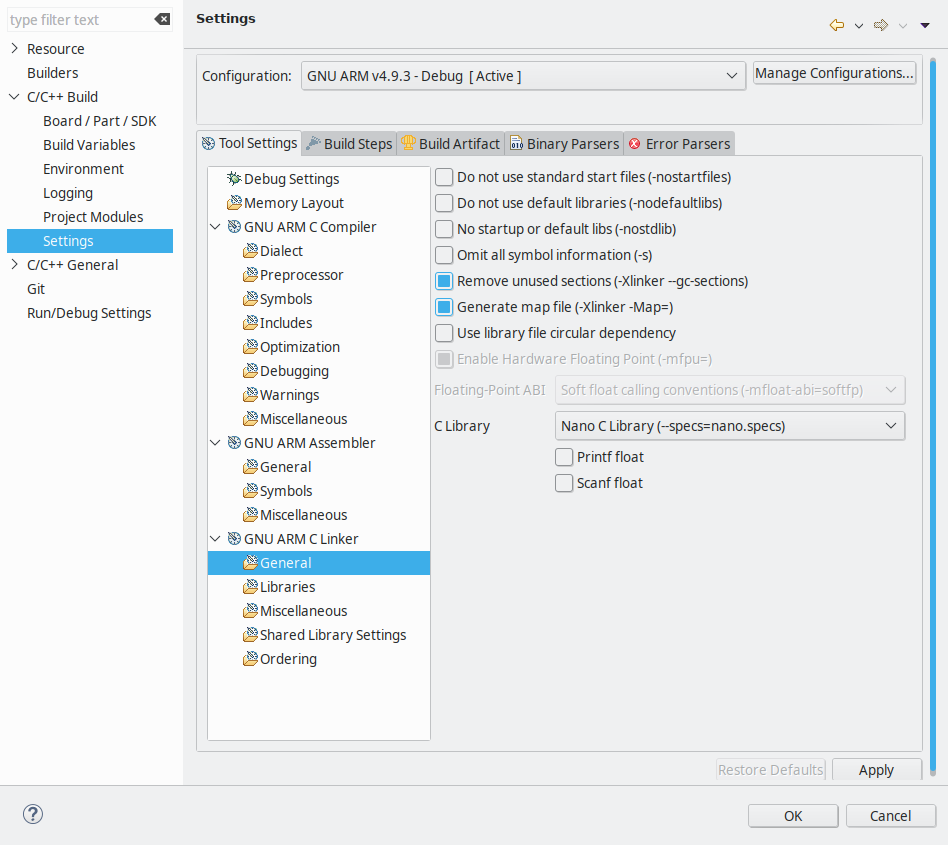
\includegraphics[width=0.85\textwidth, keepaspectratio]{imatges/SilabsPrintfFloat.png}
 \caption{Opció a {\em Simplicity} per activar el punt flotant al {\bf printf()}}
 \label{fig:SILabsPrintfFloat}
\end{figure}

Una forma força habitual de disposar dels avantatges del printf
mentre es desenvolupa i treure'l de forma ràpida quan es genera el
binari definitiu es redefinir el \textbf{printf} amb un nom nostre, i
establir una variable condicional de compilació per activar o no el
printf real, tal i com es veu en el llistat Llistat~\ref{ourprintf},
llavors en el nostre codi, enlloc de cridar \textbf{printf} per
mostrar un missatge, haurem de fer servir \textbf{PRINTF}.

\index{printf()}\index{PRINTF()}
\begin{lstlisting}[caption={Redefenir {\bf printf()}},style=customc,label=ourprintf]
#ifdef USE_PRINTF
  #define PRINTF(...) printf( __VA_ARGS__)
#else
  #define PRINTF(...)
#endif
\end{lstlisting}

\chapter{Gestió de rellotges}
\label{sec:clocks}
En la majoria de microcontroladors moderns la gestió dels rellotges és una qüestió delicada i molt important. Per tal de millorar el consum del dispositiu, és habitual tenir un control i poder decidir si cert perifèric rep el senyal de rellotge o no (més detalls a \fullref{ch:low-power}). En cas que no el rebi, el perifèric romandrà totalment desconnectat i no consumirà energia. En cas que el vulguem fer servir, una de les primeres coses que haurem de fer és activar i proporcionar-li el senyal de rellotge adequat.

Per aquesta tasca de controlar els rellotges, acostuma a existir un perifèric concret que fa tota la gestió, tant de manegar l'entrada de diferents senyals de rellotge com de preparar i enviar aquests senyals als diferents perifèrics. En els microcontroladors tant de SiliconLabs com de ST tenim diferents branques de rellotge per diferents perifèrics i la CPU. En termes generals podem dir que els perifèrics considerats lents (RTC, LEUART, etc.) reben un senyal de rellotge de baixa freqüència, els perifèrics considerats ràpids (USART, SPI, DAC, ADC, Timers, etc.) un senyal de rellotge d'alta freqüència i la CPU i els perifèrics més relacionats (DMA, Interrupcions, etc.) un altre rellotge \cite[94]{EFM32GRM}\cite[152]{STM32F4RM}.

Al llarg dels diferents exemples s'anirà veient com es gestionen els rellotges. En els casos més senzills, tant sols cal activar el rellotge pel perifèric desitjat cridant a la funció {\bf CMU\_ClockEnable()}\index{CMU{\_}ClockEnable()}. aquesta funció rep com a paràmetre el perifèric al que se li vol enviar o desactivar el rellotge.

Altres funcions permeten decidir quin senyal rellotge concret es connecta amb quina branca (funció {\bf CMU\_ClockSelectSet()}\index{CMU{\_}ClockSelectSet()}); dividir un rellotge abans d'entrar a cert perifèric ({\bf CMU\_ClockDivSet()}\index{CMU{\_}ClockDivSet()}) (Llistat~\ref{clk_mng}).

\index{CMU{\_}ClockSelectSet()}\index{CMU{\_}ClockDivSet()}\index{CMU{\_}ClockEnable()}
\begin{lstlisting}[style=customc,caption={Exemple de configuració del rellotge pel RTC},label=clk_mng]
CMU_ClockSelectSet( cmuClock_LFA, cmuSelect_LFXO ); // El rellotge "Low Frequency Crystal Oscillator" entra al bus LFA
CMU_ClockDivSet( cmuClock_RTC, cmuClkDiv_32768 );  // El rellotge es divideix per 32768 abans d'alimentar el RTC
CMU_ClockEnable(cmuClock_RTC, true);   // S'activa el rellotge pel periferic RTC
CMU_ClockEnable(cmuClock_HFLE, true );  // S'activa el rellotge "Low energy clock"
\end{lstlisting}


\section{{\em Systick}}
\label{sec:systick}
Com ja s'ha mencionat breument a \fullref{se:arquitectura}, dins els {\em cores} ARM-M hi ha un {\em timer} simple sense cap relació amb els {\em Timers} perifèrics que veurem més endavant a \fullref{sub:Timers}. Aquest {\em timer} es coneix pel nom de \gls{Systick} i consta tan sols d'un comptador decreixent de 24 bits i un generador d'interrupció en quant arriba a zero \cite[312]{GuideCortexM3M4}. El timer Systick funciona amb el rellotge de la CPU dividit per algun factor configurable. Això caldrà tenir-ho en compte alhora de fer implementacions de baix consum, on en ocasions s'atura aquest rellotge (veure~\fullref{ch:low-power}).

Aquest {\em timer} està pensat perquè els S.O. el puguin fer servir, i com que està integrat dins el {\em core} Cortex, la portabilitat dels S.O. entre diferents fabricants serà molt senzilla (seria més complicat haver de fer un port per cada {\em timer} diferent de cada fabricant).

%%ATENCIO: Trenco manualment CMU\_ClockFreqGet\\(cmuClock\_CORE) pq Latex no ho fa be
L'exemple al repositori implementa una funció de {\bf Delay()}\index{Delay()}. El que es fa és configurar el {\em Systick} perquè generi una interrupció cada 1 mil·lisegon (Llistat~\ref{systickconfig}). Com que la funció {\bf CMU\_ClockFreqGet\\(cmuClock\_CORE)}\index{CMU{\_}ClockFreqGet()} retorna la freqüència de funcionament del rellotge del sistema, al dividir-la per 1000 i configurar el Systick amb aquest valor, generarà una interrupció cada mil·lisegon.

A la ISR corresponent s'incrementa una variable global per tenir un comptatge dels mil·lisegons transcorreguts (veure Llistat~\ref{systickISR}). La variable {\bf msTicks} s'ha definit com a {\bf volatile} pel que s'explicarà a \fullref{sb:volatile}.

\index{SysTick{\_}Config()}\index{CMU{\_}ClockFreqGet()}
\begin{lstlisting}[caption={Configuració del {\em Systick}},style=customc,label=systickconfig]
main() {
  ...
  SysTick_Config(CMU_ClockFreqGet(cmuClock_CORE) / 1000);
  ...
}
\end{lstlisting}

\index{SysTick{\_}Handler()}
\begin{lstlisting}[caption={ISR del {\em Systick}},style=customc,label=systickISR]
void SysTick_Handler(void)
{
  msTicks++;       /* increment counter necessary in Delay()*/
}
\end{lstlisting}

Per últim, la funció {\bf Delay()}\index{Delay()} rep com a paràmetre els mil·lisegons a aturar-se i s'espera aquest temps comptant el temps fent servir la variable global que incrementa la ISR (Llistat~\ref{systickDelay}).

\index{Delay()}
\begin{lstlisting}[caption={Funció delay() amb {\em Systick}},style=customc,label=systickDelay]
void Delay(uint32_t dlyTicks)
{
  uint32_t curTicks;

  curTicks = msTicks;
  while ((msTicks - curTicks) < dlyTicks) ;
}
\end{lstlisting}



\chapter{GPIO}
\label{sub:GPIO_2}
Diem \gls{GPIO} al perifèric encarregat de la gestió de l'entrada i sortida de propòsit general. Fent servir aquest perifèric podrem configurar l'entrada o la sortida d'un pin concret del microcontrolador i posar-hi el valor desitjat ('0' o '1') o llegir quin valor hi ha posat algun altre dispositiu.

De forma general, un pin en concret el podrem configurar perquè treballi com a entrada o com a sortida. Si un pin està configurat com a entrada, el valor de voltatge elèctric que tingui a l'entrada del pin, es podrà llegir per part del codi del microcontrolador. De forma inversa, un pin configurat com a sortida posarà el valor elèctric equivalent al valor que el codi escrigui.

Així, si estem treballant a 3.3 Volts d'alimentació i d'entrada i sortida, si a un pin configurat com d'entrada algun altre dispositiu
hi posa un valor proper a 3.3 volts, des de el nostre software o comunament anomenat \textbf{Firmware} (\gls{FW}) en la seva forma anglesa, llegirem que aquest pin té un valor d''1'. En canvi, si el pin està configurat com a sortida, quan posem un '1' des del \gls{FW}, el pin corresponent forçarà un valor de 3.3 volts (com a la Figura~\ref{fig:led}).

\begin{remark}
 Quan diem que l'alimentació és de 3.3 Volts estem suposant aquesta tensió d'alimentació, però el rang acceptable va de 1.8 fins a 3.8 Volts i llavors les sortides tindrien el valor d'alimentació \cite[9]{EFM32TG840}. Així, si alimentem el microcontrolador a, posem per cas, 2.8 Volts, un '1' lògic de sortida d'un pin forçarà 2.8 Volts a aquell pin.
\end{remark}



\begin{figure}
 \centering
 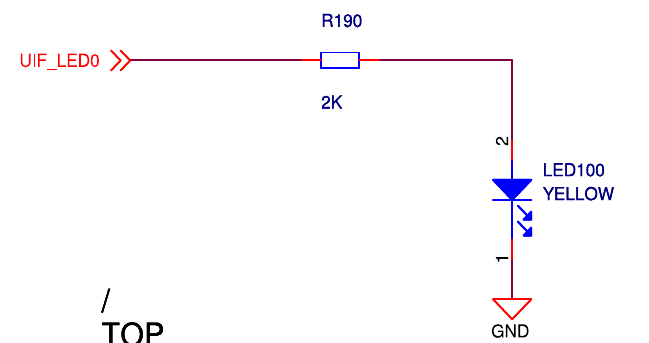
\includegraphics[width=0.85\textwidth, keepaspectratio]{imatges/led.png}
 \caption{Esquemàtic mostrant un LED connectat a un pin de GPIO}
 \label{fig:led}
\end{figure}

Existeixen diferents formes de configurar un pin segons el fabricant i la tecnologia, la més comuna és el mode {\em push-pull} que permet forçar un valor '1' o '0' segons convingui. Una altra opció que de vegades cal fer servir és el mode {\em open-drain}, que la sortida només pot forçar el valor '0' però no el valor '1'.

En aquest cas, per forçar el valor '1' es fa servir una resistència connectada a 3.3 volts; aquesta mena de resistència s'anomena un {\em \gls{pull-up}}. Aquesta mena de resistències (o el seu complementari, un {\em \gls{pull-down}}) també s'utilitza en la connexió de polsadors o botons, de manera que quan el botó no està polsat, la resistència de {\em pull-up} (o de {\em pull-down}) força el valor corresponent.

\begin{figure}
 \centering
 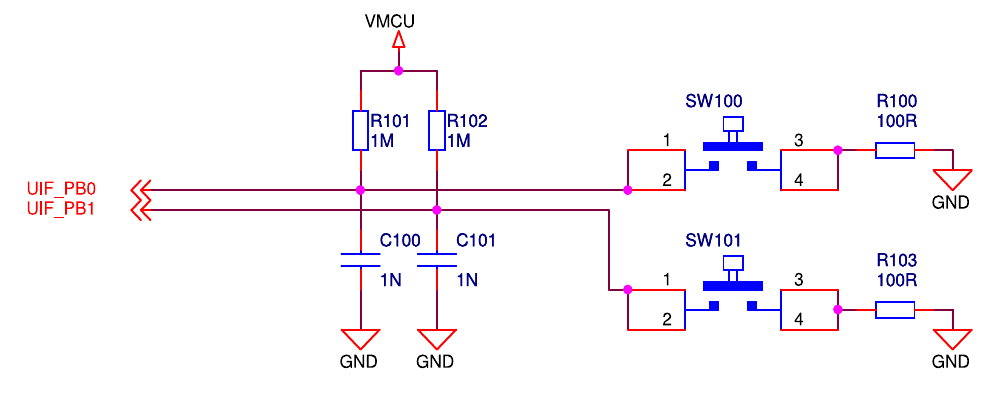
\includegraphics[width=0.85\textwidth, keepaspectratio]{imatges/buttons.png}
 \caption{Esquemàtic amb resistències de {\em pull-ups}}{Esquemàtic amb resistències de {\em pull-ups} (etiquetades com R101 i R102)}
 \label{fig:pullup}
\end{figure}

Com es veu al esquemàtic de la Figura~\ref{fig:pullup}, quan no es prem el botó les resistències etiquetades R101 i R102 fan que la línia estigui a ‘1' lògic ({\em pull-up}). En quan es prem el botó, aquest connecta GND a la línia i per tant passa a tenir el valor lògic ‘0'.

Cal saber també que la quantitat de corrent que un pin individual pot proporcionar està limitada i, en alguns casos, es pot seleccionar la quantitat màxima de corrent que pot donar un pin concret.

\section{Un exemple senzill}
\label{sub:GPIO_2_example}
Farem un codi que llegeixi l'estat dels botons de la placa, i en cas que estiguin pitjats, s'encén o apaga el LED. Veiem el codi el llistat~\ref{gpio_example}.

\begin{lstlisting}[style=customc,caption={Codi d'exemple de GPIO},label=gpio_example]
CMU_ClockEnable(cmuClock_GPIO, true);

GPIO_PinModeSet(gpioPortD,  7, gpioModePushPullDrive, 0); /* LED */
GPIO_PinModeSet(gpioPortD,  8, gpioModeInput, 0); /* Boto 0 */
GPIO_PinModeSet(gpioPortB, 11, gpioModeInput, 0); /* Boto 1 */

/* Infinite loop */
while (1) {
  if (GPIO_PinInGet(gpioPortD, 8) == 0) {
    GPIO_PinOutClear(gpioPortD, 7);
  }
  if (GPIO_PinInGet(gpioPortB, 11) == 0) {
    GPIO_PinOutSet(gpioPortD, 7);
  }
}
\end{lstlisting}

El primer que es fa amb la sentència {\bf CMU\_ClockEnable()}\index{CMU{\_}ClockEnable()} és alimentar amb un rellotge al perifèric \gls{GPIO}. En la arquitectura Cortex-M de Silicon Labs cal fer això per cada perifèric que fem servir. D'aquesta manera, un perifèric que no necessitem no rep cap rellotge i el seu consum és disminueix dràsticament.

Tot seguit es configuren els 3 pins que utilitzarem:
\begin{itemize}
 \item PD7 com sortida per controlar el LED,
 \item PD8 i PB11 com entrades connectades als botons 0 i 1.
\end{itemize}

Un cop configurats els pins, dins el bucle infinit es va mirant tota l'estona per {\em polling} el valor dels dos pins d'entrada i canviant el valor de sortida cap al LED segons toqui.


\section{BSP}
\label{sec:BSP}

Podem començar a introduir el concepte de \gls{BSP} que no són més que funcions específiques per la nostra PCB de manera que ens aïllen la implementació de la funcionalitat.

Anem a suposar que canviem de PCB (o de versió) i el LED que volem encendre ja no està connectat al pin D7 si no que està, posem per cas, al E2. Caldria canviar totes les crides que tinguéssim al nostre codi de l'estil vist al Llistat \ref{orig_gpio_bsp} per la del Llistat \ref{change_gpio_bsp} amb tots els errors que això provocar.

\begin{lstlisting}[style=customc, caption=Codi de configuració d'un pin, label=orig_gpio_bsp]
GPIO_PinOutSet(gpioPortD, 7);
\end{lstlisting}

\begin{lstlisting}[style=customc, label=change_gpio_bsp, caption=Codi amb la nova configuració del pin]
GPIO_PinOutSet(gpioPortE, 2);
\end{lstlisting}

Una forma molt habitual de treballar és escriure funcions amb les funcionalitats més comunes i que ens amaguin aquests detalls. Així, pel nostre exemple podríem definir les funcions del Llistat \ref{BSP_example}.
\index{LedInit()}\index{LedOn()}\index{LedOff()}\index{GPIO{\_}PinOutSet()}\index{GPIO{\_}PinModeSet()}\index{GPIO{\_}PinOutClear()}
\begin{lstlisting}[style=customc, label=BSP_example, caption=Exemple de BSP senzill]
LedInit() {
  GPIO_PinModeSet(gpioPortD, 7, gpioModePushPullDrive, 0); /* LED */
}

LedOn() {
  GPIO_PinOutSet(gpioPortD, 7);
}

LedOff() {
  GPIO_PinOutClear(gpioPortD, 7);
}
\end{lstlisting}

Fent servir aquestes funcions enlloc de les crides directes al GPIO ens permetran introduir canvis a la PCB sense haver de canviar gaire el nostre codi.

Habitualment en el BSP s'inclouen les inicialitzacions dels diversos rellotges (veure~{\fullref{sec:clocks}}), les funcions per accedir a recursos propis de la placa com LEDs o botons, configuració de les opcions de {\em Debug} (Veure~{\fullref{sub:console}}), etc.

\section{Manipulant bits individuals}
\label{sec:bits}

Tot i que no és específic dels GPIOs, veurem aquí com manipular bits individuals en C. Sovint ens caldrà posar a valor '0' o '1' un bit individual d'una variable sense canviar el valor de la resta dels bits, veiem aquí les receptes per fer-ho.

\begin{remark}
 La numeració de bits en C comença pel 0, així el bit menys significatiu d'una variable serà sempre el 0 i el més significatiu $N-1$, amb $N$ el nombre de bits de la variable. Per situar un 1 a un bit determinat, en C es fa servir l'operador {\bf <{}<}, que desplaça cap a l'esquerra el valor de l'esquerra tants bits com indiqui el valor de la dreta.
\end{remark}

L'exemple per aquesta secció es troba al repositori en el projecte \href{https://github.com/mariusmm/cursembedded/tree/master/Simplicity/Bit_1}{Bit\_1}.
\index{|}
\subsection{Posar a 1 un bit}
Per posar un bit concret a '1' d'una variable tant sols cal fer una OR lògica (símbol {\bf |}) tal com es veu al Llistat~\ref{example_bit}.

En aquest cas, primer es posa a '1' el bit 4 de la variable {\em my\_variable}.
\index{main()}
\begin{lstlisting}[style=customc, label=example_bit, caption=Manipulant un bit concret d'una variable]
void main(void) {
  ...
  uint8_t my_variable;
  ...
  my_variable = 5;
  // Set to '1' bit 4
  my_variable |= (1 << 4);
  printf("my_variable: 0x%02X\r\n", my_variable); // should be 0x15
  // Now set to '0' bit 2
  my_variable &= ~(1 << 2);
  printf("my_variable: 0x%02X\r\n", my_variable); // should be 0x11
  // Now we toggle bit 0 twice
  my_variable ^= (1 << 0);
  printf("my_variable: 0x%02X\r\n", my_variable); // should be 0x10
  my_variable ^= (1 << 0);
  printf("my_variable: 0x%02X\r\n", my_variable); // should be 0x11
  ...
  
  if ( (my_variable & 0x10) != 0 ) {
    /* the variable my_variable has the 4th bit set */
  }
}
\end{lstlisting}

\index{\&}\index{\~{}}
\subsection{Posar a 0 un bit}
Per posar a zero un bit individual, la feina a fer és una mica més estranya, ja que cal fer una AND lògica amb tots els bits a '1' menys el desitjat que haurà d'estar a '0'. Això es pot fer amb la mateixa construcció d'abans i fent l'operació NOT bit a bit (amb el símbol {\bf \~{}}) abans de fer la AND (símbol {\bf \&}).

En el mateix exemple es veu com, després de posar a 1 el bit 4, es posa a 0 el bit 3 amb la operació AND comentada.

\index{\^{}}
\subsection{{\em Toggle} un bit}
Per a fer un {\em toggle} d'un bit individual, el que cal fer és la operació lògica XOR (símbol {\bf \^{}}) amb el bit desitjat al valor '1'.

A l'exemple es fa {\em toggle} dues vegades al bit 0 de la variable.

\subsection{Comparar si un bit està a cert valor}
L'altre necessitat que apareix sovint és la de comprovar el valor d'un bit determinat d'una variable.

L'opció més habitual és fer una AND lògica entre la variable i el bit interessant i comprovar que el resultat és diferent de '0'. Si la comparació dona cert vol dir que el bit en qüestió està a '1', en cas contrari, el bit d'interès té el valor '0'. Es pot veure al final de l'exemple al Llistat~\ref{example_bit}, on es comprova que el bit 4 de la variable sigui valgui '1'.

\begin{remark}
Aquesta mena d'operacions són força propicies per introduir {\em bugs} complicats de detectar. Operar per error un bit que no pertany a aquella mida de variable pot portar a errors molt difícils de detectar i el compilador no donarà cap mena de error o avís.
\end{remark}


\chapter{Controlador d'interrupcions}
\label{ch:IRQ}
Una interrupció (\gls{IRQ}) és un succés que interromp l'execució normal del processador i passa a executar un codi de programa especial pel succés concret. La \gls{ISR} és el codi que es crida per a cada succés o interrupció.

Cada interrupció té assignada una ISR pròpia. Aquesta informació s'acostuma a guardar en una zona de memòria especial, anomenada memòria de vectors d'interrupció.

Les IRQs estan enumerades i tenen prioritats, així habitualment, un valor menor vol dir major prioritat. Aquest valor de IRQ també es fa servir per saber quina posició dels vectors d'interrupció es troba la ISR corresponent.

El controlador d'interrupcions gestiona quines interrupcions rebudes arriben al processador, segons les prioritats i si la interrupció concreta està activada o no.

Veurem un cas amb els GPIO, el codi està disponible \href{https://github.com/mariusmm/cursembedded/tree/master/Simplicity/GPIO_2}{al repositori} . En aquest cas, el que es fa primer és configurar els pins perquè generin una interrupció HW al flanc de baixada (recordem el {\em pull-up} a la PCB, Figura~\ref{fig:pullup}). Tot seguit s'activen les interrupcions corresponents.
\index{NVIC{\_}EnableIRQ()}\index{GPIO{\_}IntConfig()}
\begin{lstlisting}[style=customc]
 /* Set Interrupt configuration for both buttons */
GPIO_IntConfig(gpioPortD, 8, false, true, true);
GPIO_IntConfig(gpioPortB, 11, false, true, true);

/* Enable interrupts */
NVIC_EnableIRQ(GPIO_EVEN_IRQn);
NVIC_EnableIRQ(GPIO_ODD_IRQn);
\end{lstlisting}

En el cas dels Cortex-M de SiliconLabs, els pins de \gls{GPIO} poden generar només 2 interrupcions, els pins parells la interrupció GPIO\_EVEN\_IRQ i els pins senars la GPIO\_ODD\_IRQ \cite[405]{EFM32GRM}. En els microcontroladors de ST, hi ha una arquitectura diferent i cada pin d'entrada pot generar una IRQ segons el seu índex de manera que el pin PA2, el PB2, el PC2 etc. generen la IRQ EXTI2, però només un d'aquests pins pot generar la IRQ \cite[384]{STM32F4RM}.

En el cos de l'exemple, com que els botons estan connectats al pin D8 i B11 cada un d'ells activarà una de les dues interrupcions.

La \gls{ISR} per la interrupció parell la veiem al Llistat~\ref{gpio_isr}.
\index{GPIO{\_}EVEN{\_}IRQHandler()}\index{GPIO{\_}IntClear()}\index{GPIO{\_}IntGet()}\index{GPIO{\_}PinOutClear()}
\begin{lstlisting}[style=customc, label=gpio_isr, caption=Exemple d'ISR per GPIO]
void GPIO_EVEN_IRQHandler(void) {
  uint32_t aux;

  aux = GPIO_IntGet();

  /* clear flags */
  GPIO_IntClear(aux);

  /* Set LED off */
  GPIO_PinOutClear(gpioPortD, 7);
}
\end{lstlisting}

A l'arquitectura Cortex-M el nom de les ISR està fixat en un fitxer de l'entorn de programació, de manera que només cal escriure una funció amb el nom correcte i ja tenim definida la ISR. El fitxer que defineix les ISR depèn de cada model de microcontrolador, en el nostre cas és el fitxer startup\_efm32tg.S.

En el cas de l'arquitectura Cortex, la pròpia ISR ha de netejar el \gls{flag} d'interrupció que l'ha cridat. Això es fa al principi de tot de la \gls{ISR}, llegint quins \glspl{flag} estan actius (funció {\bf GPIO\_IntGet()}\index{GPIO\_IntGet()}) i tot seguit netejant aquests mateixos \glspl{flag} ({\bf GPIO\_IntClear()}\index{GPIO\_IntClear()}).

A continuació, s'encén o s'apaga el LED segons correspongui (a una ISR s'apaga, a l'altre s'encén).

L'altre cosa a destacar d'aquest exemple és el que hi ha dins el bucle infinit, que està buit. I està buit perquè, en aquest exemple, el microcontrolador no té res a fer fins que no hi hagi una interrupció provinent d'un botó.

En una aplicació real, en aquest bucle es podrà posar codi que si s'hagi d'executar contínuament, o instruccions que posin “a dormir” el microcontrolador tot esperant una interrupció, etc. Tot això ho anirem veient més endavant.

\section{Escrivint ISRs en C}
\label{sec:IRQ_example}
Com ja sabem, les \gls{ISR} són les funcions especials que s'executen tant bon punt es dispara una interrupció determinada.

Tradicionalment les adreces a aquestes \glspl{ISR} (anomenats de vegades vectors d'interrupció) s'emmagatzemaven a una zona especial de la memòria del processador. Quan el processador rebia una \gls{IRQ}, com que aquestes van numerades simplement calcula l'offset de la IRQ a la taula de ISRs i executa aquella funció determinada.

En els ARM Cortex amb els que treballem això es fa tal qual acabem d'explicar (link a la documentació d'ARM). En el cas dels Cortex (i la majoria de microcontroladors i processadors) la taula de vectors d'interrupcions es col·loca a la posició 0 de memòria.

El que cal, doncs, és que les nostres eines de compilació posin aquests vectors com toca a cada un dels binaris que generem. En el cas de les eines per Cortex (tant Simplicity com les eines de ST ho fan així), aprofiten un codi d'inicialització proporcionat per ARM anomenat, en el nostre cas startup\_efm32tg.S. Aquest fitxer està escrit en assemblador i, entre d'altres coses, té el codi que es veu a la Figura~\ref{fig:ISR}:

\begin{figure}
 \centering
 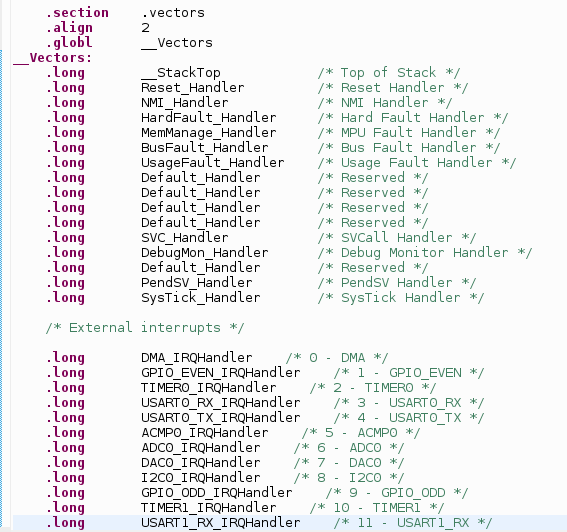
\includegraphics[width=0.85\textwidth, keepaspectratio]{imatges/interruptvectorcortex.png}
 \caption{Vectors d'interrupció}
 \label{fig:ISR}
\end{figure}

Com es pot veure, aquest codi declara el nom de les ISRs corresponents a cada una de les IRQs possibles al microcontrolador. Més endavant en el mateix fitxer, es posa una funció per defecte per a cada una de les ISR que és només un bucle sense fi. Com que aquesta funció es declara com {\em weak}, nosaltres podrem sobreescriure–la en cas que ho vulguem fer.

En el cas de Cortex, les funcions de ISR no han de ser definides de cap forma especial, més enllà de posar el nom que li correspongui.

En altres arquitectures, com ara AVR d'Atmel, les ISR han de retornar d'una manera diferent a les funcions normals donat que durant la crida a una ISR no es guarden tots els registres com es fa a una crida a una funció normal. Si escrivim la funció en assemblador, enlloc d'una instrucció {\bf RET} ens caldrà escriure una instrucció {\bf RETI}.

Si estem treballant en llenguatge C, com que el compilador posa una instrucció {\bf RET} quan acaba la funció, caldrà indicar-li d'alguna forma que la funció en qüestió és una ISR i que ha d'acabar-la amb una instrucció {\bf RETI}.

Això, en el cas d'AVR es fa com es veu al Llistat \ref{ISR_AVR_1} o \ref{ISR_AVR_2} depenent del tipus de compilador que estiguem fent servir.

\begin{lstlisting}[style=customc, label=ISR_AVR_1, caption=Exemple d'ISR per AVR]
#pragma vector=TIMER0_OVF_vect
__interrupt void MotorPWMBottom() {
  // codi
}
\end{lstlisting}

\begin{lstlisting}[style=customc, label=ISR_AVR_2, caption=Exemple d'ISR per AVR]
ISR(PCINT1_vect) {
  //codi
}
\end{lstlisting}


\section{Fent servir ISRs}
Com ja hem comentat, una \gls{ISR} s'executa quan es dispara una \gls{IRQ}. Durant l'execució de la ISR el microcontrolador està en un mode d'execució especial, amb les demés IRQs desactivades (depèn de l'arquitectura això pot no ser així).

Donat que la resta d'IRQs poden estar desactivades, és important que el temps que el processador estigui executant una ISR sigui el mínim possible i que el codi, per tant, sigui el més senzill possible.

Si el que hem de fer, a part de tasques molt simples a la ISR, és engegar o controlar un procés més complicat, aquest procés no el farem dins la ISR, si no en un procés a part i comunicarem via \glspl{flag}, cues, semàfors o mecanismes similars la ISR amb el procés. Així minimitzem el temps que el processador està en mode ISR.

\subsection{Ús de variables globals}
\label{sb:volatile}
Com ja hem vist breument a \fullref{sub:memory-mapped} hi ha una paraula reservada que es fa servir quan es fan accessos a memòria i altres usos d'una variable on el compilador no ha d'actuar amb cap optimització. La paraula reservada {\bf volatile} davant la declaració d'una variable indica al compilador que la variable s'hi ha d'accedir tal com diu el codi i no efectuar cap optimització.

\begin{remark}
En el cas de modificar el valor d'una variable global des d'una ISR, cal declar-la com a {\bf volatile}.
\end{remark}

\chapter{Timers}
\label{sub:Timers}
Un {\em \gls{Timer}} (temporitzador) és un dels perifèrics més habituals de trobar en un microcontrolador. Bàsicament consisteix en un comptador que pot generar alguna interrupció quan arriba a un cert llindar o al seu valor límit. Com sempre, cada fabricant el fa segons el seu criteri i, per tant, cada un té característiques diferents.

Normalment els {\em timers} es poden connectar a diferents rellotges disponibles dins el microcontrolador. A més, força sovint els {\em timers} poden dividir prèviament la freqüència del rellotge que l'alimenta per reduir-la encara més. Així, podem tenir un rellotge d'1 MHz alimentant un {\em timer} que abans de que hi entri es divideixi per 8 per tenir un rellotge efectiu de 125 kHz. Amb això, si configurem el {\em timer} perquè compti fins al valor 125000, tindrem que el {\em timer} generarà una interrupció cada segon.

En el cas de Silicon Labs, els Timers tenen múltiples opcions \cite[249]{EFM32GRM}:

\begin{itemize}
 \item comptador de 16 bits
 \item pre-escalatge del rellotge: el rellotge d'entrada es pot pre-escalar (dividir) per diversos factors (de 2 fins a 1024).
 \item diverses fonts de rellotge
 \item diverses formes de comptatge (cap a munt, cap avall, amunt i avall, etc.)
 \item 3 canals per Timer, per generar diverses interrupcions (per {\em overflow}, per arribar a un llindar, {\em underflow}, etc.)
\end{itemize}



Tot plegat fa que sigui força complicat de configurar, i com ve sent costum, el fabricant ens dona una biblioteca per simplificar-nos una mica la vida.

Els controls que tenim habitualment per un Timer, un cop configurat, són \cite{EMLIB}:

\begin{itemize}
 \item engegar i parar el Timer ({\bf TIMER\_Enable()}\index{TIMER{\_}Enable()} a EMLIB).
 \item llegir o configurar el màxim valor pel timer ({\bf TIMER\_TopGet()}\index{TIMER{\_}TopGet()} / {\bf TIMER\_TopSet()}\index{TIMER{\_}TopSet()} a EMLIB).
 \item llegir o configurar el valor pel compare ({\bf TIMER\_CompareGet()}\index{TIMER{\_}CompareGet()} / {\bf TIMER\_CompareSet()}\index{TIMER{\_}CompareSet()} a EMLIB).
\end{itemize}

Els usos que li podem donar a aquest perifèric són variats, els més habituals són els següents::
\begin{itemize}
 \item Comptar el temps: es configura per a que generi una interrupció cada segon i ja tenim un rellotge de temps real. Hi ha perifèrics específics per aquesta tasca (\glspl{RTC}) com es veurà a \fullref{sub:RTC}.
 \item Fer {\em delays} acurats: de vegades cal que un senyal o una acció passi després d'un cert temps. Amb un Timer ben configurat podem comptar temps petits de l'ordre de microsegons.
 \item Comptar polsos externes: segons quins Timers poden comptar segons una entrada externa, i aquesta no cal que sigui un rellotge. Pot ser, per exemple, les pulsacions d'un botó o les transicions d'un senyal.
 \item Generar senyals \gls{PWM}: tipus de senyal digital per controlar motors o d'altres dispositius (Veure~{\fullref{sub:PWM}}).
\end{itemize}

\section{Exemple senzill amb un Timer}
\label{sub:Timers_exemple}
El \href{https://github.com/mariusmm/cursembedded/tree/master/Simplicity/Timer_1}{primer exemple} fa servir un Timer per esperar-se 1 segon a canviar d'estat el LED (fer un {\em toggle}) després que es premi el Botó 0.

El que es fa en primer lloc és configurar el Timer0 amb un seguit d'opcions. Les més importants de cara a l'exemple són:
\begin{itemize}
 \item .prescale = timerPrescale1024 que configura el divisor de rellotge a 1024.
 \item .mode = timerModeUp així el Timer només compta cap amunt.
 \item .oneShot = true en aquest cas, un cop arribi al màxim valor el Timer es pararà.
\end{itemize}

Un cop configurat el Timer, s'entra en el bucle infinit.
Dins el bucle infinit, si es polsa el botó 0, es posa el comptador del Timer a 0 i s'engega el comptador (Llistat~\ref{Timer_example_1}).
\index{TIMER{\_}CounterSet()}\index{TIMER{\_}Enable()}\index{main()}\index{GPIO{\_}PinInGet()}
\begin{lstlisting}[style=customc, label=Timer_example_1, caption=Codi d'exemple d'ús d'un Timer ]
void main(void) {
  ...
  if (GPIO_PinInGet(gpioPortD, 8) == 0) {
    TIMER_CounterSet(TIMER0, 0);
    TIMER_Enable(TIMER0, true);
  }
}
\end{lstlisting}

Tot seguit, es comprova si el comptador ha arribat al valor {\bf TOP\_VALUE} usant la funció {\bf TIMER\_CounterGet()}\index{TIMER{\_}CounterGet()}, si és així es fa {\em toggle} del LED (s'encén si estava apagat o el contrari), s'atura el Timer i es posa el seu comptador a 0 (Llistat~\ref{Timer_example_2}).

\index{main()}\index{TIMER{\_}CounterGet()}\index{TIMER{\_}Enable()}\index{TIMER{\_}CounterSet()}\index{GPIO{\_}PinOutToggle()}
\begin{lstlisting}[style=customc, label=Timer_example_2, caption=Codi per comprovar si el Timer ha arribat a cert valor]
void main(void) {
  ...
  /* If timer count gets to TOP_VALUE, toggle LED and stop Timer */
  if (TIMER_CounterGet(TIMER0) >= TOP_VALUE) {
    GPIO_PinOutToggle(gpioPortD, 7);
    TIMER_Enable(TIMER0, false);
    TIMER_CounterSet(TIMER0, 0);
  }
  ...
}
\end{lstlisting}

Com hem calculat el valor {\bf TOP\_VALUE} (13671)?

\begin{verbatim}
Rellotge d'entrada al Timer: 14.000.000 Hz (14 MHz)
Prescaler: 1024 (Seleccionat al inicialitzar el timer)
Freqüència de treball del Timer = 14.000.000 / 1024 = 13.671,875 Hz
\end{verbatim}

Per tant, en un segon el comptador del Timer haurà comptat fins a 13.671 (o 13.672, no ve d'un tick!).

En aquest exemple hem fet servir el Timer d'una forma força rudimentària, ja que no és gaire habitual fer {\em polling} d'un Timer per transcorre un temps determinat. Es fa servir aquest mètode per implementar funcions tipus {\bf Delay()} simples. A continuació veurem un exemple més complicat basat en interrupcions.

\section{Exemple més complex amb el Timer}
\label{sub:Timers_exemple_2}
Al \href{https://github.com/mariusmm/cursembedded/tree/master/Simplicity/Timer_2}{segon exemple} fem servir interrupcions
per obtenir informació del Timer i així alliberar la CPU.

Primer de tot, cal saber per quines condicions pot generar interrupcions el nostre Timer. En el cas de la família EFM32, cada Timer té només una interrupció (anomenada TIMERn\_IRQn) però tenen els següents esdeveniments que poden generar una interrupció \cite{EFM32GRM}:

\begin{itemize}
 \item {\em Overflow}: quan el comptador arriba a {\bf TOP}
 \item {\em Underflow}: quan el comptador arriba a 0
 \item {\em Compare Match}: quan el comptador arriba a un valor determinat. N'hi ha un per cada canal del Timer.
\end{itemize}

Així doncs, quan estiguem a la \gls{ISR} del Timer si hem activat més d'un esdeveniments a que generi la interrupció haurem de mirar quin esdeveniments ha estat.

El Timer es configura igual que a l'exemple anterior, i a més s'activen les interrupcions per aquest perifèric amb el codi que es veu a \ref{Timer_enableIRQ}.
\index{TIMER{\_}IntEnable()}\index{NVIC{\_}EnableIRQ()}
\begin{lstlisting}[style=customc, label=Timer_enableIRQ, caption=Codi corresponent a l'activació de les IRQs del Timer]
 /* Enable overflow interrupt */
TIMER_IntEnable(TIMER0, TIMER_IF_OF);

/* Enable IRQ for Timer 0*/
NVIC_EnableIRQ(TIMER0_IRQn);
\end{lstlisting}

Amb això, un cop s'engegui el Timer i quan arribi el comptador a {\bf TOP} llençarà la interrupció {\bf TIMER0\_IRQn}, que executarà la {\bf ISR TIMER0\_IRQHandler()}\index{TIMER0{\_}IRQHandler()} que es veu al Llistat~\ref{Timer_IRQ} on simplement es netegen els \glspl{flag} d'interrupció i es fa {\em toggle} del \gls{LED}.
\index{TIMER{\_}IntGet()}\index{TIMER{\_}IntClear()}
\begin{lstlisting}[style=customc, label=Timer_IRQ, caption=ISR del Timer]
void TIMER0_IRQHandler(void) {
  uint32_t flags;

  /* Clear flag for TIMER0 */
  flags = TIMER_IntGet(TIMER0);
  TIMER_IntClear(TIMER0, flags);

  /* Toggle LED ON/OFF */
  GPIO_PinOutToggle(gpioPortD, 7);
}
\end{lstlisting}

La configuració i la posada en marxa del Timer es fa a la \gls{ISR} del botó 0, de manera similar a com ja havíem fet anteriorment a d'altres exemples: primer es netegen els {\em flags} de la \gls{IRQ}, tot seguit es posa el comptador del Timer a 0, es posa el valor màxim i per últim s'engega el Timer (Llistat~\ref{GPIO_ISR_Timer}).

\index{GPIO{\_}EVEN{\_}IRQHandler()}\index{GPIO{\_}IntGet()}\index{GPIO{\_}IntClear()}
\index{TIMER{\_}CounterSet()}\index{TIMER{\_}TopSet()}\index{TIMER{\_}Enable()}
\begin{lstlisting}[style=customc, label=GPIO_ISR_Timer, caption=ISR del GPIO per l'exemple del Timer]
void GPIO_EVEN_IRQHandler(void) {
  uint32_t flags;

  /* clear flags */
  flags = GPIO_IntGet();
  GPIO_IntClear(flags);

  /* Set counter to 0  */
  TIMER_CounterSet(TIMER0, 0);

  /* Set TIMER Top value */
  TIMER_TopSet(TIMER0, TOP_VALUE);

  /* Start Timer */
  TIMER_Enable(TIMER0, true);
}
\end{lstlisting}

Per últim, fer notar que al bucle infinit final del {\bf main()}\index{main()} no hi ha cap codi, ja que la \gls{CPU} no té res a fer mentre espera la pulsació del botó o que s'exhaureixi el temps, En el tema de baix consum (\fullref{ch:low-power}) es veurà com aprofitar aquest fet per reduir el consum del sistema amb un exemple a \fullref{sub:letimer_example}.

\chapter{RTC}
\label{sub:RTC}

Un altre perifèric que acostumem a trobar als microcontroladors actuals és una mena de \gls{Timer} una mica especial. Habitualment aquests perifèrics serveixen per tenir un control de temps en segons i/o un calendari, enlloc de temps molts més curts de mil·lisegons o microsegons com els Timers que ja hem vist.

Aquest tipus de perifèrics acostumen a fer servir una entrada de rellotge pròpia de 32,768 kHz (32.768 Hz), que és una freqüència de rellotge molt habitual per aquestes feines. Algunes famílies de microcontroladors poden funcionar amb altres freqüències o generar-la internament per fer el sistema més senzill.

Els RTC varien força de fabricant a fabricant, així els STM32 tenen un RTC complet, on podem guardar dia, mes i any, hora minut i segons i el dispositiu mateix manté la data (dies del mes, anys de traspàs, etc.), fent molt senzill mantenir una data dins el dispositiu (veure Figura~\ref{fig:STRTC}) \cite[799]{STM32F4RM}.

\begin{figure}
 \centering
 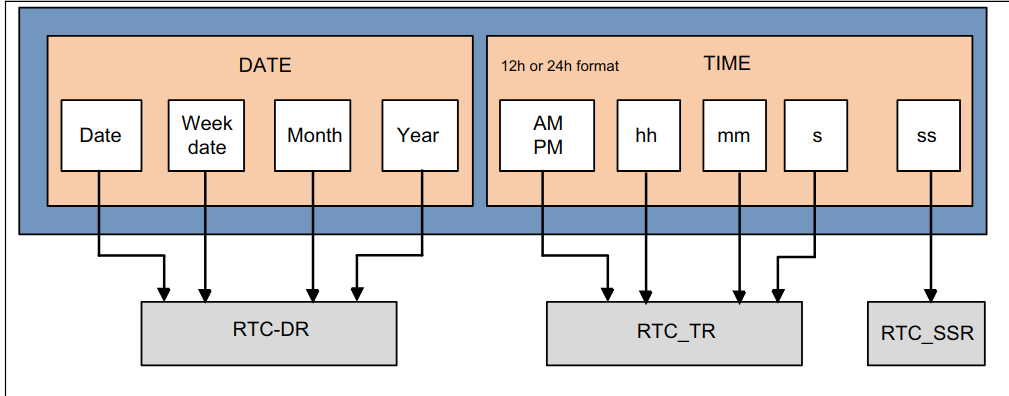
\includegraphics[width=0.85\textwidth, keepaspectratio]{imatges/RTC_STM32.png}
 \caption{Registres del RTC de STM32 \cite{ST_AN3371}}
 \label{fig:STRTC}
\end{figure}

Per contra, els RTCs de EFM32 són força més senzills, i és, de fet, un Timer de 24 bits de molt baix consum amb una entrada de rellotge pròpia i que es pot triar cada quan generen una interrupció \cite[285]{EFM32GRM}. Si triem fer una interrupció cada segon, podem manegar per SW la gestió de l'hora i el calendari.

\href{https://github.com/mariusmm/cursembedded/tree/master/Simplicity/RTC}{A l'exemple per EFM32} tant sols se selecciona el rellotge de 32 kHz extern (LFXO), el divisor a 32768 per tenir un tic cada segon i es configura per a que generi una interrupció cada 2 segons (veure Llistat~\ref{RTCInit}. En aquest exemple, a la \gls{ISR} només es canvia el LED (s'apaga o encén segons el seu estat actual) (veeure Llistat~\ref{RTCISR}).

\index{CMU{\_}ClockSelectSet()}\index{CMU{\_}ClockDivSet()}\index{NVIC{\_}EnableIRQ()}
\index{RTC{\_}CompareSet()}\index{RTC{\_}IntEnable()}\index{NVIC{\_}ClearPendingIRQ()}
\begin{lstlisting}[style=customc, caption={Inicialització del RTC}, label=RTCInit]
void main(void) {
  ...
  CMU_ClockSelectSet( cmuClock_LFA, cmuSelect_LFXO );
  CMU_ClockDivSet( cmuClock_RTC, cmuClkDiv_32768 );
  ...

  RTC_CompareSet(0, 2);

  /* Enabling Interrupt from RTC */
  RTC_IntEnable(RTC_IFC_COMP0);
  NVIC_ClearPendingIRQ(RTC_IRQn);
  NVIC_EnableIRQ(RTC_IRQn);
  ...
}
\end{lstlisting}

\index{RTC{\_}IRQHandler()}\index{RTC{\_}IntClear()}\index{GPIO{\_}PinOutToggle()}
\begin{lstlisting}[style=customc,caption={ISR del RTC},label=RTCISR]
void RTC_IRQHandler(void) {
  /* Clear interrupt source */
  RTC_IntClear(RTC_IFC_COMP0);

  GPIO_PinOutToggle(gpioPortD, 7);
}
\end{lstlisting}


Si volguéssim mantenir un rellotge fent servir aquest perifèric podríem configurar-lo perquè generi una interrupció cada segon, i dins la \gls{ISR} mantenir un comptador de segons i actualitzar la data segons això.

\section{RTC externs}
Quan la majoria de microcontroladors no incloïen un RTC intern com els que hem vist, era habitual fer servir un dispositiu \gls{RTC} extern. D'aquests dispositius n'hi ha de tota mena però la majoria tenen les següents característiques:

\begin{itemize}
 \item Interface \gls{I2C} (veure \fullref{sub:I2C}) amb el microcontrolador.
 \item Necessita un cristall de 32.768 Hz.
 \item Un error d'aproximadament un segon a l'any.
 \item Actualitza data i hora, calculant anys de traspàs.
 \item Capacitat de generar interrupcions segons una alarma programable.
 \item Molt baix consum i alimentació separada amb bateria (pila botó).
 \item Molts d'ells tenen una petita memòria RAM adreçable per guardar-hi dades persistents.
\end{itemize}

Amb aquesta mena de dispositiu, el microcontrolador es descarrega de gestionar el calendari i només cal accedir als registres del RTC extern per saber l'hora o data del sistema. A la majoria dels casos també és possible programar alguna mena d'alarma, de forma que quan arriba cert temps o data una línia dedicada pot generar una interrupció al microcontrolador. Alguns models també tenen la possibilitat de generar un senyal de forma periòdica per tenir, per exemple, un senyal a 128 Hz.

Habitualment l'alimentació d'aquests dispositius es pot fer per un canal separat de l'alimentació principal i usant una bateria o pila tipus botó. Això permet que el RTC sempre estigui alimentat encara que es perdi l'alimentació principal (per avaria, tall de corrent, canvi de bateries, etc.). Aprofitant que sempre tenen alimentació, força RTCs tenen una zona de memòria RAM per a que el microcontrolador pugui guardar-hi dades persistents. L'accés a aquesta zona de memòria també es fa mitjançant el bus \gls{I2C}, sent molt senzill emmagatzemar-hi dades.

Per últim, cal dir que són dispositius força barats (entre 0.5 € i 3 € per unitat en volums petits), sent una bona opció en cas que el nostre microcontrolador no disposi d'aquesta funcionalitat \cite{RTCDS1}\cite{RTCDS2}\cite{RTCDS3}.

\chapter{PWM}
\label{sub:PWM}
El \gls{PWM} és una tècnica per aconseguir controlar la potència subministrada a un dispositiu mitjançant un senyal digital. Simplificant, fent que un senyal digital (‘1' o ‘0') estigui més o menys estona a ‘1' aconseguim controlar la potència que rep el dispositiu a la sortida.

Aquest tipus de modulació es fa servir per controlar motors simples (motors DC) on enlloc d'enviar un voltatge variable per controlar la velocitat enviem un senyal PWM. Així, si enviem polsos més llargs el motor girarà més ràpid i si enviem polsos més curts el motor girarà més a poc a poc. Com que el voltatge que se li envia sempre es el màxim, la potència del motor és sempre la màxima.

Els dos paràmetres principals d'un senyal PWM són la seva freqüència i el seu \gls{duty cycle} (la durada del pols a ‘1' respecte la durada del pols a ‘0').

\href{https://github.com/mariusmm/cursembedded/tree/master/Simplicity/PWM_1}{A l'exemple} es fa servir el LED de la placa enlloc d'un motor. Posarem una freqüència molt petita, així la podrem veure amb els nostres ulls, i anirem canviant el \gls{duty cycle} amb els dos botons, de manera que podem veure què està passant.

Primer veiem què passa i després veiem com ho fa el codi.

Només programar la placa veiem el LED fent pampallugues força ràpid tota l'estona. Si polsem el botó 1 veurem que el LED va més ràpid, si tornem a polsar el botó 1 encara va més ràpid així fins que al cinquè cop que el polsem el LED es queda encès tota l'estona.

El que estem veient és que el LED va rebent un senyal PWM on el duty cycle cada cop és més gran (més estona encès que apagat) fins que al final és del 100\% (sempre encès). El ritme al que fa pampallugues el LED és (més o menys) la freqüència del PWM, que en aquest exemple és de 13.5~Hz.

\section{Generar PWM}
\label{sub:PWM_example}

La majoria de microcontroladors actuals tenen algun dispositiu HW que permet generar \gls{PWM}. En el cas dels micros de Silicon Labs, el dispositiu que ens permet generar-ne són els \glspl{Timer}.

Un Timer (veure la secció~\fullref{sub:Timers}) no és més que un comptador HW que genera interrupcions o sortides quan el comptador arriba a uns certs valors.

Per generar PWM, el Timer es configura el seu registre {\bf TOP} per a que ens doni la freqüència de funcionament del PWM desitjada. El que farà el Timer és comptar sempre fins a TOP i re-iniciar-se en quan hi arribi. Per generar el \gls{duty cycle} el que es fa es posar el valor desitjat al registre {\bf COMPARE} ({\bf CC}). El que farà el Timer és treure un ‘1' mentre el comptador no arribi a {\bf CC}, llavors posarà un ‘0' a la sortida fins que el comptador arribi a {\bf TOP}, on tornarà a començar el cicle (Figura~\ref{fig:pwm_timer})..

\begin{figure}
 \centering
 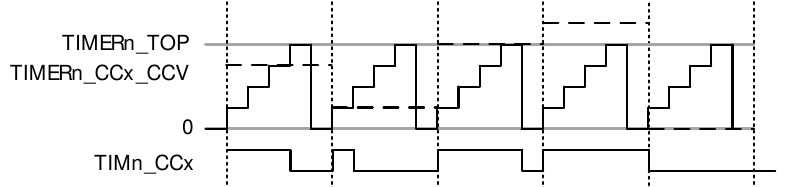
\includegraphics[width=0.85\textwidth, keepaspectratio]{imatges/pwm_timer.png}
 \caption{Generació de PWM amb un timer \cite[262]{EFM32GRM}}
 \label{fig:pwm_timer}
\end{figure}
En el codi d'exemple (Llistat \ref{Set_Timer_PWM}), el que es fa és configurar el TIMER1 en mode PWM i connectar la sortida del Timer al Pin D7 que és on està el LED connectat.

\index{TIMER{\_}InitCC()}
\begin{lstlisting}[style=customc, label=Set_Timer_PWM, caption=Configuració del Timer per l'exemple PWM]
 /* Set Timer */
TIMER_InitCC(TIMER1, 1, &timerCCInit);
TIMER1->ROUTE |= (TIMER_ROUTE_CC1PEN | TIMER_ROUTE_LOCATION_LOC4);
\end{lstlisting}

A continuació és configuren els dos registres importants per generar PWM (Llistat~\ref {Timer_PWM_Conf}). Com que volem una freqüència baixa pel \gls{PWM} per poder veure'l amb els nostres ulls, al registre {\bf TOP} hi posem {\bf PWM\_FREQ} (4000), que el calculem de la següent manera \cite{EFM32GRM}.
\begin{displaymath}
\text{Freq. de PWM} = \frac{\text{Freq Clk}}{\text{prescaler} * \text{valor TOP}} = \frac{14.000.000 \text{ Hz}}{256 * (4000 +1 )} = 13.67 \text{ Hz}
\end{displaymath}

\index{TIMER{\_}TopSet()}\index{TIMER{\_}CompareBufSet()}
\begin{lstlisting}[style=customc, label=Timer_PWM_Conf, caption=Configuració del Timer per l'exemple PWM]
TIMER_TopSet(TIMER1, PWM_FREQ);
TIMER_CompareBufSet(TIMER1, 1, pwm_value);
\end{lstlisting}

La resta del codi és senzill: es preparen les dues interrupcions per cada un dels botons, i quan algun dels dos es prem, la \gls{ISR} modifica el valor del registre {\bf CC} del Timer (un botó augmenta el duty cycle, l'altre el disminueix).

Si veiem el senyal generada amb un oscil·loscopi veiem el que es mostra a la Figura~\ref{fig:DutyCycle1} (estat per defecte).
\begin{figure}
 \centering
 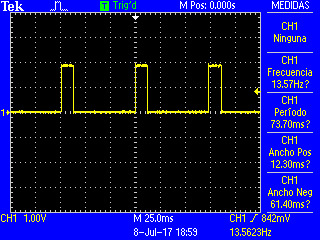
\includegraphics[width=0.85\textwidth, keepaspectratio]{imatges/DutyCycle1.png}
 \caption{PWM amb Duty Cycle al 16\%}
 \label{fig:DutyCycle1}
\end{figure}

Veiem que la freqüència real del senyal és de 13.57 Hz (73.70 ms de període) i que el senyal està a ‘1' 12.30 ms i a ‘0' a 61.40 ms.

Segons anem pitjant el botó 1 i anem augmentant el \gls{duty cycle} anem veient com està més estona a '1' el senyal (Figures~\ref{fig:DutyCycle2},
\ref{fig:DutyCycle3} i \ref{fig:DutyCycle4}).
Cal fixar-se que la freqüència no varia, sempre és \~13.5 Hz i el que va variant és l'estona que està a ‘0' o a ‘1' el senyal.

\begin{figure}
 \centering
 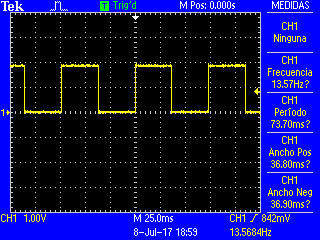
\includegraphics[width=0.85\textwidth, keepaspectratio]{imatges/DutyCycle2.png}
 \caption{PWM amb Duty Cycle al 50\%}
 \label{fig:DutyCycle2}
\end{figure}

\begin{figure}
 \centering
 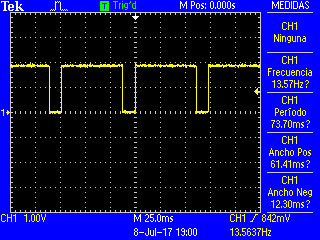
\includegraphics[width=0.85\textwidth, keepaspectratio]{imatges/DutyCycle3.png}
 \caption{PWM amb Duty Cycle al 83.3\%}
 \label{fig:DutyCycle3}
\end{figure}

\begin{figure}
 \centering
 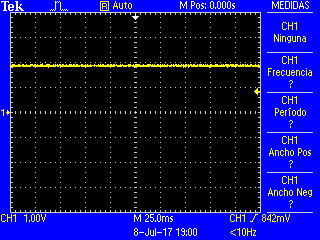
\includegraphics[width=0.85\textwidth, keepaspectratio]{imatges/DutyCycle4.png}
 \caption{PWM amb Duty Cycle al 100\%}
 \label{fig:DutyCycle4}
\end{figure}

Per acabar, es pot provar de canviar la freqüència del \gls{PWM} per a que no es vegi el LED fent pampallugues. Cal augmentar la freqüència a un valor que superi els 100Hz i enlloc de veure el LED encendre's i apagar-se, es veurà com varia la intensitat amb la que llueix.

\chapter{\em Watchdog}
\label{sec:Watchdog}
En els microcontroladors actuals tenim un perifèric amb un funcionament força peculiar. Quan s'activa el {\em \gls{Watchdog}}, aquest comença a comptar un cert període de temps, i si no “s'alimenta”, reiniciarà tot el sistema \cite[123]{EFM32GRM}\cite[709]{STM32F4RM}.

I per què volem un perifèric que ens reinici el nostre sistema? Doncs per si el nostre \gls{FW} té algun error i es queda penjat (està en un {\em \gls{dead-lock}}, en un bucle sense sortida, etc.), sempre serà millor que el sistema s'iniciï de nou. Imaginem el cas d'un marcapassos (un sistema encastat força crític); què és millor? Que es quedi penjat per un error del \gls{FW} que passa molt poc (si passés sovint s'hauria detectat) o que quan passi aquest error el sistema es reinici i torni a funcionar en menys de, posem, un segon?

I com evitem que si tot va be el {\em watchdog} no ens reiniciï el sistema? Doncs “alimentant-lo” de tant en tant de manera que el comptador intern del {\em Watchdog} torni a zero (Figura~\ref{fig:Watchdog}).

\begin{figure}
 \centering
 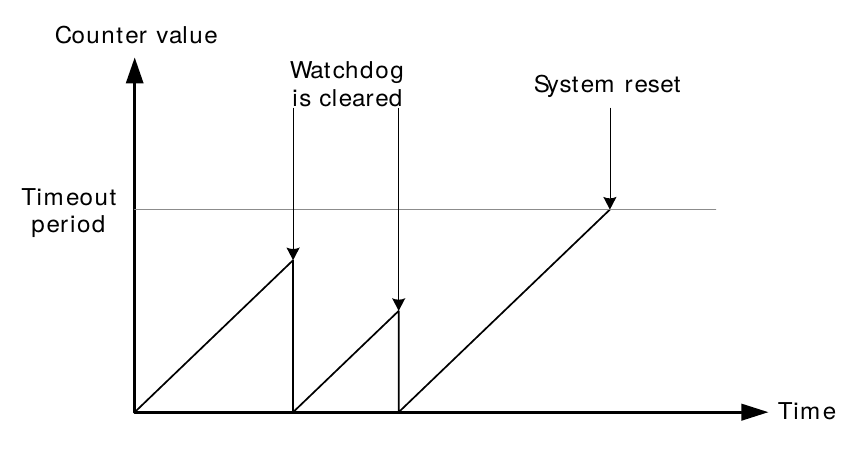
\includegraphics[width=0.85\textwidth, keepaspectratio]{imatges/Watchdog.png}
 \caption{Funcionament del {em Watchdog} \cite{EFM_AN0015}}
 \label{fig:Watchdog}
\end{figure}

La majoria de fabricants ens donen unes poques funcions per treballar amb el {\em Watchdog} (en el cas de Silicon Labs a la biblioteca EMLIB tenim el mòdul em\_wdog). Habitualment hi ha alguna funció per configurar-lo, una per engegar-lo i una per alimentar-lo. Hi ha fabricants que no permeten deshabilitar el {\em Watchdog} un cop s'ha engegat per assegurar-se que cap error de \gls{FW} provocarà que deixi de funcionar.
\index{WDOG{\_}Feed()}
\begin{lstlisting}[style=customc]
WDOG_Feed();
\end{lstlisting}

Habitualment es pot triar quina és la freqüència de funcionament del {\em Watchdog}, per tenir més o menys temps abans no reiniciï el sistema; normalment de pocs mil·lisegons fins a algunes desenes de segons.

\section{Exemple}
\label{sub:Watchdog_example}
En l'\href{https://github.com/mariusmm/cursembedded/tree/master/Simplicity/Watchdog}{exemple que hi ha al repositori}
es configura el {\em Watchdog} perquè treballi amb un rellotge intern de 1 kHz i que compti fins a 4097, de manera que si ningú alimenta el {\em Watchdog} en 4 segons, aquest reiniciarà el sistema. L'exemple conté un bucle que va fent blinkar el LED de la placa i una \gls{ISR} que quan es prem el botó 0 alimenta el {\em Watchdog} (Llistat~\ref{WatchdogISR}).

\index{GPIO{\_}EVEN{\_}IRQHandler()}\index{GPIO{\_}IntGet()}\index{GPIO{\_}IntClear()}\index{WDOG{\_}Feed()}
\begin{lstlisting}[style=customc,caption={ISR del botó que alimenta el {\em Watchdog}},label=WatchdogISR]
void GPIO_EVEN_IRQHandler(void) {
  uint32_t aux;

  aux = GPIO_IntGet();
  /* clear flags */
  GPIO_IntClear(aux);

  /* Feed watchdog */
  WDOG_Feed();
}
\end{lstlisting}

Si no premem el botó abans no passin 4 segons, el sistema es reiniciarà. I com ho veurem a l'exemple? Doncs perquè el codi el primer que fa és esbrinar per què s'està reiniciant el sistema (Llistat~\ref{Check_boot}). Si ha estat perquè ha entrat el {\em Watchdog}, el LED no blinkarà.

\begin{lstlisting}[style=customc,caption={Codi per detectar la causa del reinici},label=Check_boot]
if (resetCause & RMU_RSTCAUSE_WDOGRST) {
  resetbyWatchdog = true;
} else {
  resetbyWatchdog = false;
}
\end{lstlisting}

Cal tenir en compte que aquest dispositiu serveix per solucionar possibles fallades totals del sistema, així que cal ser curosos amb el seu ús. Així, si tenim un bucle {\bf for} que pot generar algun problema, no te sentit posar la comanda de {\em touch} al {\bf watchdog} dins del {\bf for}, si no que segurament te sentit fer-ho abans i després del bucle.

\part{Programació de perifèrics II}
\label{part:programacio_2}

\chapter{ADC}
\label{sub:ADC}
%% AMPLIAR
Un perifèric força habitual en els microcontroladors actuals és l'\gls{ADC}.

Aquesta perifèric el que fa és llegir un senyal analògic (un voltatge) i convertir-lo a un valor digital (un número). Hi ha diversos models d'\gls{ADC} amb característiques diferents, però bàsicament les característiques principals d'un ADC són:
\begin{itemize}
 \item Resolució: fa referència a quants bits dona la conversió de l'ADC. Un ADC de 16 bits, en principi, dona més detall del senyal d'entrada que un ADC de 8 bits. Actualment el més habitual és trobar ADCs d'entre 8 i 16 bits de resolució.
 \item {\em Sampling rate}: és la cadència amb la que l'ADC agafa una nova mostra del senyal i la converteix a digital. Els microcontroladors actuals incorporen ADCs que poden arribar al milió de mostres per segon.
 \item referència: pot ser que es compari el senyal segons una referència determinada i el ADC ens doni el valor respecte a aquesta referència.
\end{itemize}

En els microcontroladors moderns, és habitual que davant de l'ADC hi hagi un multiplexor analògic, de manera que es pugui convertir diverses senyals connectades a diferents pins amb un mateix perifèric.

A l'hora de fer servir un \gls{ADC}, caldrà configurar-lo en els paràmetres de funcionament que necessitem per la nostra senyal.

Com la majoria de perifèrics, l'ADC pot generar una o vàries \glspl{IRQ} segons certes condicions, habitualment quan s'ha acabat la conversió. D'aquesta manera la CPU no cal que faci {\em polling} del registre d'estat per saber si la conversió ha finalitzat.

\section{Exemple d'ADC}
\label{sub:ADC_example}
\href{https://github.com/mariusmm/cursembedded/tree/master/Simplicity/ADC_1s}{Per aquest exemple} ens cal per primer cop un petit HW addicional. Farem servir un potenciòmetre que ens donarà una tensió entre Vdd i 0 volts segons el seu recorregut. La sortida d'aquest potenciòmetre la connectarem al pin 16 del connector de Debug de la PCB. Els altres dos pins aniran a 19 i 20 del mateix connector (veure esquemàtic a la Figura~\ref{fig:sch_adc} i fotografia del sistema a Figura~\ref{fig:setup_adc}).

\begin{figure}
 \centering
 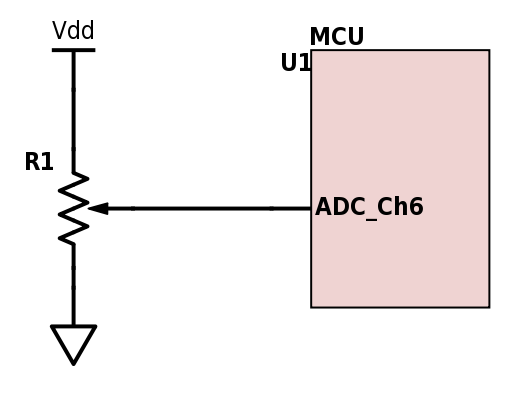
\includegraphics[width=0.85\textwidth, keepaspectratio]{imatges/adc_schematic.png}
 \caption{Esquemàtic de la connexió del Potenciòmetre al canal d'\gls{ADC}}
 \label{fig:sch_adc}
\end{figure}

\begin{figure}
 \centering
 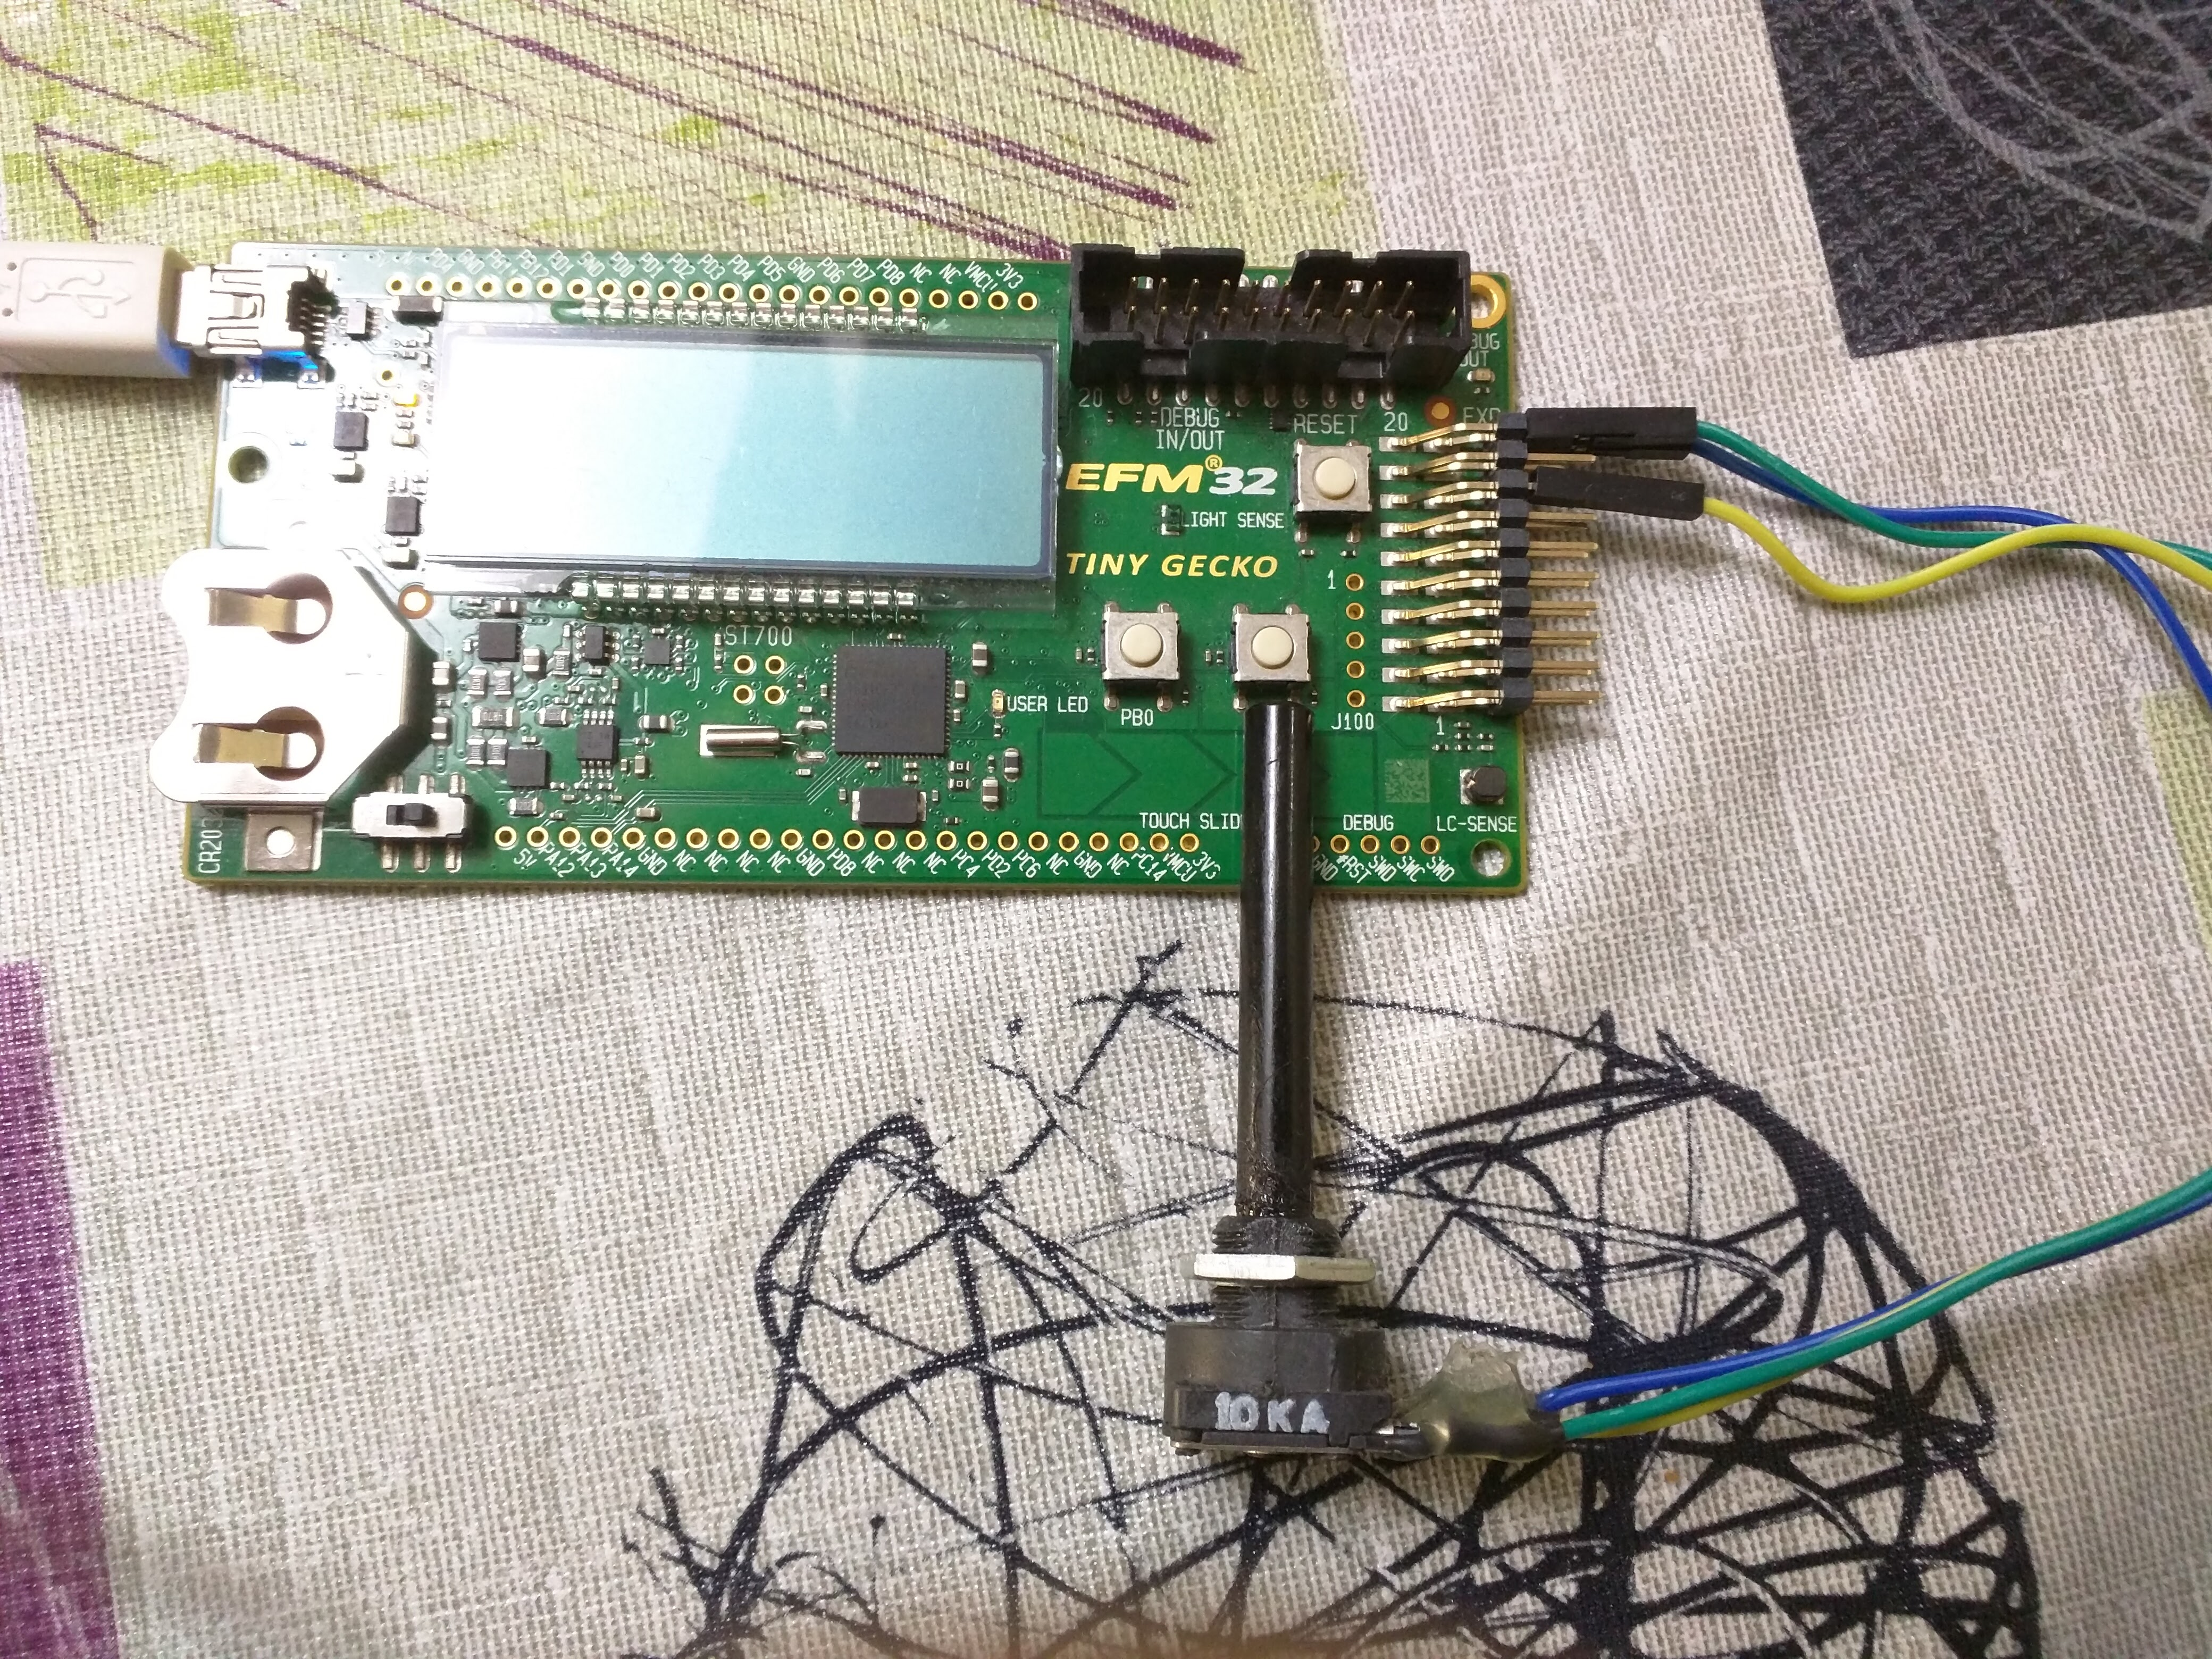
\includegraphics[width=0.85\textwidth, keepaspectratio]{imatges/adc_setup.png}
 \caption{Fotografia del sistema amb el connexitat correcte}
 \label{fig:setup_adc}
\end{figure}

Connectat així el potenciòmetre, quan estigui a un extrem del recorregut tindrem 0V a l'entrada de l'ADC i quan estigui a l'altre extrem hi tindrem \gls{Vdd}.

A l'exemple trobem un codi molt senzill, on simplement s'inicia l'\gls{ADC} amb els paràmetres per defecte i només es canvia el canal d'entrada (el 6) i la tensió de referència (en aquest cas Vdd).

D'aquesta manera, els 12 bits de resolució del ADC serviran per comparar la tensió d'entrada amb els 3.3 V amb els que està alimentat el microcontrolador a la placa.

\begin{remark}
 Els 3.3 Volts és el voltatge de funcionament de la placa d'avaluació. Els ADC normalment poden mesurar tensions fins a la seva tensió d'alimentació i és per això que en aquest cas podem mesurar fins a 3.3 Volts. Si l'alimentació fos menor, el rang de treball de l'ADC també ho seria. En el cas particular de l'ADC dels EFM32, poden tenir voltatges fixes com a referència \cite[378]{EFM32GRM}.
\end{remark}

El codi, un cop inicialitzat el ADC, realitza les següents accions:
\index{ADC{\_}Start()}\index{ADC{\_}DataSingleGet()}
\begin{lstlisting}[frame=single,caption={Codi de lectura de l'ADC},style=customc]
while (1) {
  ADC_Start(ADC0, adcStartSingle);
  while (ADC0->STATUS & ADC_STATUS_SINGLEACT);
  ADCvalue = ADC_DataSingleGet(ADC0);
  printf("ADC Value %lu\r\n", ADCvalue);
}
\end{lstlisting}

El que fan aquests 4 línies és:
\begin{itemize}
 \item Engegar l'ADC i que comenci una conversió
 \item Esperar a que la conversió finalitzi consultant el registre STATUS de l'ADC.
 \item Llegir el valor de la conversió feta per l'ADC.
 \item Imprimir per la consola de {\em Debug} el valor de la conversió.
\end{itemize}

Per tant, el que veurem un cop engeguem l'exemple serà com es van imprimint els valors llegits per l'\gls{ADC}. Si anem movent el potenciòmetre veurem que els valors van canviant des de 0 fins a 4095.

\chapter{DAC}
\label{sub:DAC}
Un \gls{DAC} és un dispositiu que es pot veure com l'invers d'un ADC, ja que a partir d'unes dades digitals genera un senyal analògic equivalent. Els paràmetres de funcionament d'un DAC són, doncs, molt similars als del seu perifèric germà l'\gls{ADC}.

Al {\em datasheet} de la família amb la que treballem \cite[421]{EFM32GRM} hi ha la descripció, bastant breu, de les característiques principals d'aquest perifèric. Bàsicament, té un registre anomenat {\bf CHxDATA} on s'ha d'escriure el valor que volem que es converteixi a voltatge segons la fórmula següent\footnote{Pel cas single-ended, pel cas diferencial veure \cite[424]{EFM32GRM}}:
\begin{equation}
\label{eq:DACFormula}
 V_{OUT} = V_{Ref} \times \frac{CHxDATA}{4096}
\end{equation}

On $V_{Ref}$ és el voltatge de referència, que en aquest cas pot ser 2.5 o 1.25 Volts o la tensió d'alimentació Vdd.

\section{Exemple senzill amb el DAC}
\label{sec:DAC_Example_1}

Al \href{https://github.com/mariusmm/cursembedded/tree/master/Simplicity/DAC_1}{repositori} hi ha un exemple senzill usant el DAC per generar una tensió continua segons un valor donat.
Primer s'inicialitzarà el \gls{DAC} i la resta de perifèrics (en aquest cas els GPIO i poc més). Es configuren els botons com sempre, amb les dues interrupcions ja conegudes ({\bf GPIO\_ODD\_IRQHandler()}\index{GPIO{\_}ODD{\_}IRQHandler()} i {\bf GPIO\_EVEN\_IRQHandler()}\index{GPIO{\_}EVEN{\_}IRQHandler()}).

La part important de l'exemple és la inicialització del DAC, tal com es veu al Llistat~\ref{DACConfig}.

\index{CMU{\_}ClockEnable()}\index{DAC{\_}PrescaleCalc()}\index{DAC{\_}Init()}\index{DAC{\_}InitChannel()}
\begin{lstlisting}[style=customc, caption=Inicialització del DAC, label=DACConfig]
static void DACConfig(void) {
  /* Use default settings */
  DAC_Init_TypeDef init = DAC_INIT_DEFAULT;
  DAC_InitChannel_TypeDef initChannel = DAC_INITCHANNEL_DEFAULT;

  /* Enable the DAC clock */
  CMU_ClockEnable(cmuClock_DAC0, true);

  /* Set prescale for 500 KHz */
  init.prescale = DAC_PrescaleCalc(500000, 0);

  /* Set reference voltage to Vdd */
  init.reference = dacRefVDD;

  /* Initialize the DAC and DAC channel #1 */
  DAC_Init(DAC0, &init);
  DAC_InitChannel(DAC0, &initChannel, 1);
}
\end{lstlisting}

En aquest codi, primer es posen els valors per defecte que ens ofereix el fabricant i tant sols es modifiquen alguns paràmetres. Primer s'activa el {\em clock} del sistema cap al perifèric, tot seguit es tria el {\em prescaler} segons la freqüència de funcionament desitjada.  Després es selecciona que la referència per crear el senyal de sortida es basi en el voltatge d'entrada ({\bf dacRefVDD}). Per últim es configura el DAC i el canal (en aquest el 1 per la sortida que hem triat).

Les \gls{ISR} dels dos botons el que fan es incrementar o decrementar una variable global que serà el valor que s'enviarà al DAC per a que generi el senyal. Aquest increment o decrement es fa en passos de {\bf DAC\_STEP} unitats. D'aquesta manera pitjant els botons podrem seleccionar quin voltatge es genera a la sortida del DAC.

Dins el bucle infinit de la funció {\bf main()} (Llistat~\ref{DACMain}) s'envia el valor de la variable global cap al DAC amb la funció {\bf DAC\_ChannelOutputSet()}\index{DAC{\_}ChannelOutputSet()}, es treu el valor per la consola de debug i s'espera a que un \gls{flag} indiqui que hi ha hagut un canvi en el valor de la variable global.

\index{DAC{\_}ChannelOutputSet()}\index{printf()}\index{main()}
\begin{lstlisting}[style=customc, caption=Bucle infinit del DAC, label=DACMain]
void main(void) {
  while (1) {
    DAC_ChannelOutputSet(DAC0, 1, DACvalue);
    printf("DAC Value %lu (0x%06X)\r\n", (uint32_t) DACvalue, (uint32_t) DACvalue);
    while(signal == false);
    signal = false;
  }
}
\end{lstlisting}

Si mesurem el voltatge de sortida amb un multímetre, oscil·loscopi o analitzador lògic (que tingui entrada analògica) podem veure com els valors de la variable provoquen el canvi en voltatge esperat segons la Fórmula~\ref{eq:DACFormula} tal com es veu a la Taula~\ref{tb:DACVoltages}. El pin de sortida del DAC està connectat al pin PB12, connectat al pin 13 del connector d'expansió. La Taula~\ref{tb:DACVoltages} es registren tots els valors possible de la variable {\bf DACvalue} i el voltatge mesurat amb un multímetre digital; la tercera columna presenta la diferència entre el voltatge de la fila i l'anterior, com es pot veure cada pas corresponent a poc més de 200 mV, tal com surt a la fórmula~\ref{eq:DACFormula}. A la última fila es calcula la mitjana aritmètica de tots aquestes diferències.


\begin{table}
\caption{Taula resum dels valors mesurats del DAC}
\centering
\begin{tabular}{|c|c|c|}
\hline
{\bf Variable} & {\bf Voltatge (mV)} & {\bf Pas}\\
\hline
0 & 0 & - \\
256	& 204 & 204 \\
512	& 410 & 206 \\
768	& 614 & 204 \\
1024	& 824 & 210 \\
1280	& 1032 & 208 \\
1536	& 1238 & 206 \\
1792	& 1442 & 204 \\
2048	& 1651 & 209 \\
2304	& 1855 & 204 \\
2560	& 2060 & 205 \\
2816	& 2260 & 200 \\
3072	& 2470 & 210 \\
3328	& 2670 & 200 \\
3584	& 2880 & 210 \\
3840	& 3090 & 210 \\
4096	& 3290 & 200 \\
\hline
\multicolumn{2}{|c|}{\bf Mitjana de Pas} & 205,5 \\
%  Mitja & 205.5\\
\hline
\end{tabular}
\label{tb:DACVoltages}
\end{table}

L'exemple presentat és força bàsic i serveix per introduir la llibreria {\bf emlib} i el perifèric. A continuació veurem un exemple més complicat.

\section{Exemple més complicat amb el DAC}
\label{sec:DAC_Example_2}
En \href{https://github.com/mariusmm/cursembedded/tree/master/Simplicity/DAC_2}{aquest exemple} es farà servir el \gls{DAC} per generar un senyal periòdic tipus triangular (en anglès {\em Triangle wave}).

Es fa servir un {\em timer} per tenir una base de temps. El {\em timer} es configura a 1 kHz, dividint el rellotge d'entrada (14 MHz) entre 16 amb el {\em pre-escaler} i configurant el valor d'{\em overflow} a 875 perquè generi un senyal cada 1 mil·lisegon. Així, tindrem un nou valor cada 1 mil·lisegon i el senyal es repeteix cada 33 mostres, per tant tindrem un senyal periòdic de 30,30 Hz aproximadament (veure Equació ~\ref{eq:F_DAC_2}).

\begin{equation}
\label{eq:F_DAC_2}
 F_{senyal} = \frac{1000}{33} = 30,30 Hz
\end{equation}

El DAC es configura de la mateixa manera que a l'exemple anterior, en mode continu, amb referència al voltatge d'alimentació \gls{Vdd}. El {\em timer} es configura de manera molt similar a l'exemple vist a \fullref{sub:Timers_exemple_2}, activant les interrupcions per tenir la ISR executant-se cada 1 mil·lisegon.

A la \gls{ISR} del {\em timer} es calcula el nou valor pel \gls{DAC} i s'escriu el nou valor calculat (veure Llistat~\ref{DAC_2_Example}).

\index{TIMER0{\_}IRQHandler()}\index{DAC{\_}ChannelOutputSet()}
\begin{lstlisting}[style=customc, caption=Part de la ISR del Timer per generar la dada pel DAC, label=DAC_2_Example]
void TIMER0_IRQHandler(void) {
  ...
  if (direction_up == true) {
    DACvalue += DAC_STEP;
    if (DACvalue >= 0x1000) {
      DACvalue = 0x0FFF;
      direction_up = false;
    }
  } else {
    DACvalue -= DAC_STEP;
    if (DACvalue < 0) {
      DACvalue = 0;
      direction_up = true;
    }
  }
  DAC_ChannelOutputSet(DAC0, 1, DACvalue);
}
\end{lstlisting}

A l'hora d'executar el codi, si es connecta un oscil·loscopi o analitzador lògic al pin 13 del connector d'expansió de la placa de desenvolupament, que es correspon al pin PB12 del microcontrolador es veurà el senyal com es mostra a la Figura~\ref{fig:DAC_result}. Es pot observar com cada esglaó dura 1 mil·lisegon i els increments són de 200 mV aproximadament (Figura~\ref{fig:DAC_result_zoom}).

\begin{figure}
 \centering
 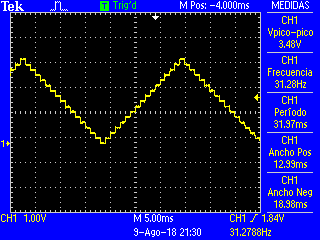
\includegraphics[width=0.65\textwidth, keepaspectratio]{imatges/DAC_result_osc}
 \caption{Senyal capturat per l'oscil·loscopi.}
 \label{fig:DAC_result}
\end{figure}

\begin{figure}
 \centering
 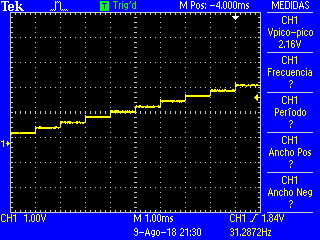
\includegraphics[width=0.65\textwidth, keepaspectratio]{imatges/DAC_result_osc_zoom}
 \caption{Detall del senyal capturat per l'oscil·loscopi, es pot veure que la unitat de temps és d'1 mil·lisegon.}
 \label{fig:DAC_result_zoom}
\end{figure}

En aquest exemple s'ha presentat com generar un senyal periòdic mitjançant el \gls{DAC} i un {\em Timer}, aquesta combinació de perifèrics és força habitual per generar senyals d'aquesta mena donada la seva senzillesa i facilitat d'ús.

En cas que els valors del senyal estiguessin pre-calculats i emmagatzemats en una taula, la \gls{ISR} del {\em Timer} només caldria agafar el següent valor de la taula.

\chapter{UART}
\label{sub:UART}
El port sèrie es encara un dels ports d'entrada i sortida més comuns de trobar en un microcontrolador i en un sistema encastat. Encara avui multitud de dispositius fan servir aquest port per rebre o enviar dades i, per tant, els microcontroladors acostumen a incloure uns quants d'aquests ports.

Aquest port sèrie en els microcontroladors el gestiona un perifèric anomenat \gls{USART} (o \gls{UART}). El port sèrie habitual, basat en l'estàndard RS-232 només té dos fils, un per rebre dades (RX) i un per enviar-ne (TX). La velocitat i les característiques de la transmissió es poden configurar i habitualment s'envien 8 bits per caràcter amb 1 bit d'stop i sense paritat (tot i que es pot canviar). Les velocitats de transmissió més habituals són: 9600 \gls{bps}, 19200 bps, 56700 bps i 115200 bps. El que cal, com és obvi, és configurar el port sèrie del microcontrolador amb els mateixos paràmetres que el dispositiu extern que estiguem usant.

L'altre aplicació pràctica del port sèrie és poder connectar el microcontrolador a un ordinador personal per poder interactuar amb ell, ja sigui per enviar dades, informació d'estatus o rebre comandes o paràmetres de configuració. Com que actualment la majoria d'ordinadors no tenen un port sèrie, s'han popularitzat molt uns petits dispositius que converteixen el port sèrie en un \gls{USB} de tipus sèrie. Aquest dispositiu el \gls{CP2102} i en parlarem més endavant..

\section{Fent servir una USART}
Com que la configuració d'un port sèrie és una mica complicada, sobretot perquè segons la velocitat de funcionament del rellotge del sistema caldrà dividir i multiplicar aquest senyal fins a tenir una velocitat adequada per la velocitat seleccionada pel port sèrie, els fabricants acostumen a donar-nos biblioteques que ens ajuden.

Dins la biblioteca acostumen a oferir una funció per enviar dades ({\bf USART\_Tx()}\index{USART{\_}Tx()}) i una per rebre'n ({\bf USART\_RX()}\index{USART{\_}Rx()}). Aquestes funcions són molt senzilles, i permeten enviar un sol byte o rebre'n un, o espera-se indefinidament fins que n'arribi un. Això pot ser que no sigui l'ideal per la nostra aplicació i les \gls{USART} permeten generar interrupcions segons certs esdeveniments. Normalment els més usats són el de byte rebut i el de byte enviat. D'aquesta manera, ens podem muntar una biblioteca que ens permeti rebre dades pel port sèrie fent servir exclusivament interrupcions i a la nostra aplicació agafem el que s'hagi rebut quan vagi bé.

La manera més habitual d'implementar aquest mecanisme asíncron de enviar o rebre dades pel port sèrie és mitjançant un \gls{buffer circular}. D'aquesta manera, la \gls{ISR} de recepció ({\bf USART1\_RX\_IRQ\\Handler()}\index{USART1{\_}TX{\_}IRQHandler()}) insereix la nova dada rebuda al {\em buffer} de recepció cada cop que la criden. Només cal escriure una funció a la nostra biblioteca que extregui un caràcter del {\em buffer} cada cop que la cridin i escriure una funció que retorni el nombre de caràcters disponibles al {\em buffer} (veure Llistat \ref{UARTISRs}).

La ISR de transmissió ({\bf USART1\_TX\_IRQHandler()}\index{USART1{\_}TX{\_}IRQHandler()}) es crida cada cop que s'acaba d'enviar un caràcter, per tant la ISR pot enviar un caràcter del {\em buffer} circular de transmissió cada cop que la cridin (quan s'ha acabat d'enviar el caràcter anterior) i ens cal una funció que copiï les dades a enviar cap al {\em buffer} circular de transmissió i engegui el procés.

\index{USART{\_}IntClear()}\index{USART{\_}Send()}\index{USART{\_}Rx()}
\begin{lstlisting}[style=customc,caption={ISRs de TX i RX de la UART},label=UARTISRs]
void USART1_TX_IRQHandler(void) {
  USART_IntClear( USART1, USART_IEN_TXC);
  USART_Send(USART1);
}

void USART1_RX_IRQHandler(void) {
  char data;

  if (USART1->IF & LEUART_IF_RXDATAV) {
    data = USART_Rx(USART1);
    PushData(data, &RX_SerialBuffer);
    USART_IntClear( USART1, USART_IEN_RXDATAV);
  }
}
\end{lstlisting}



\section{Exemple d'ús d'una UART}
\label{sub:UART_example}
Per fer les proves caldrà tenir a mà un dispositiu \gls{CP2102}. Aquest dispositiu conté un xip, el CP2102 que per un costat té un port sèrie i per l'altre un port USB de tipus {\em Virtual COM Port Device} que qualsevol ordinador, ja sigui Windows, GNU/Linux o Mac reconeixen com un port sèrie. D'aquesta manera, fent servir aquest dispositiu podem connectar un microcontrolador amb un port sèrie a un ordinador de sobretaula o portàtil que tingui un port \gls{USB} lliure.

Ara el que cal és preparar-ho tot: preparar el codi, connectar el mòdul CP2102 a la nostra placa de prototipat i connectar-la per USB a un ordinador.

El \href{https://github.com/mariusmm/cursembedded/tree/master/Simplicity/UART_1}{codi que hi ha al repositori} primer configura la USART1 del microcontrolador perquè funcioni a 115200 bps, 8 bits per caràcter, sense paritat i 1 bit d'stop, que ve a ser la configuració estàndard d'un port sèrie. També en el mateix bloc configura els dos pins del port (TX i RX). També configura com s'ha d'enrutar la USART1, en aquest cas cap la localització 1 que es correspon als pins PD0 i PD1 del microcontrolador, que estan connectats al connector d'expansió, als pins 4 i 6 respectivament (veure Figura~\ref{fig:CP2102}). Tot seguit s'envia un caràcter ‘A' pel port sèrie.

A continuació es configuren els dos botons perquè generin una \gls{IRQ}. A les \glspl{ISR} tant sols es canvia el LED (un botó l'encén i l'altre l'apaga) i un botó envia una ‘A' i l'altre botó envia un ‘B'.

Per veure aquests caràcters al nostre ordinador, primer cal connectar el mòdul CP2102 a la nostra placa pel connector d'expansió tal com es veu a la foto. Un cop connectem el CP2102 al nostre ordinador, cal engegar algun programa de terminal pel port sèrie, tipus {\em putty} \cite{putty}, {\em minicom}, {\em Tera Term} \cite{teraterm}, etc.

\begin{remark}
 També es pot instal·lar un terminal dins del {\bf Simplicity Studio}. Cal anar a l'{\em Eclipse Marketplace}, buscar el {\bf TM Terminal} i instal·lar-lo \cite{tmterminal}. Així tindrem el terminal integrat dins el IDE.
\end{remark}

\begin{figure}
 \centering
 \includegraphics[width=0.85\textwidth, keepaspectratio]{imatges/img_20180302_162857.png}
 \caption{Connexió del CP2102 a la placa de prototipat}
 \label{fig:CP2102}
\end{figure}


\section{Un exemple amb la UART més complicat}
\label{sec:UART_example_2}
Un cop vist un exemple senzill de com es configura una USART, anem a fer un exemple més complex, rebent i enviant dades del microcontrolador cap al PC i a l'inrevés. El codi està al \href{https://github.com/mariusmm/cursembedded/tree/master/Simplicity/UART_2}{repositori}.

En aquest cas farem servir \glspl{buffer circular} per guardar les dades rebudes o a enviar.  És una implementació senzilla d'un buffer circular sense gaire secrets, l'hem posat a la biblioteca {\bf CircularBuffer}. Aquesta biblioteca ofereix unes funcions molt senzilles per gestionar el buffer circular:
\begin{itemize}
 \item {\bf PushData()}\index{PushData()} que permet inserir un caràcter al {\em buffer}
 \item {\bf PopData()}\index{PopData()} que retorna el següent caràcter del {\em buffer}
 \item {\bf AvailableData()}\index{AvailableData()} que indica la quantitat de caràcters disponibles al {\em buffer}
\end{itemize}

En aquest exemple es fan servir les interrupcions de la USART per controlar-la, de manera que al rebre un caràcter, la \gls{ISR} corresponent l'insereix al {\em buffer} corresponent (hi ha dos {\em buffer}, un de recepció i un d'enviament), veure Llistat~\ref{ISR_UARTRX_Avançada} i \ref{ISR_UARTTX_Avançada}.
\index{USART1{\_}RX{\_}IRQHandler()}\index{USART{\_}Rx()}\index{USART{\_}IntClear()}
\begin{lstlisting}[style=customc,label=ISR_UARTRX_Avançada,caption=Exemple ISR avançada]
void USART1_RX_IRQHandler(void) {
  char data;

  if (USART1->IF & LEUART_IF_RXDATAV) {
    data = USART_Rx(USART1);
    PushData(data, &RX_SerialBuffer);
    USART_IntClear( USART1, USART_IEN_RXDATAV);
  }
}
\end{lstlisting}

D'aquesta manera, en qualsevol moment que es rebi un caràcter per la UART, la \gls{ISR} el guardarà el {\em buffer} {\bf RX\_SerialBuffer} i seguirà l'execució el nostre programa.

Quan calgui, podrem cridar a la funció {\bf AvailableData()}\index{AvailableData()} per saber si hem rebut alguna cosa i processar-la si cal.

Per enviar dades, cal que primer omplim el \gls{buffer circular} corresponent ({\bf TX\_SerialBuffer}) amb el que vulguem enviar i després cridar la funció {\bf USART\_Send()}\index{USART{\_}Send()}. D'aquesta manera, i gràcies a que hem configurat la USART perquè llenci una \gls{IRQ} cada cop que acabi d'enviar un caràcter, la USART enviarà un primer caràcter i es cridarà la ISR, que tornarà a cridar la funció d'enviar un caràcter fins que no en quedi cap més al {\em buffer}.

\index{USART1{\_}TX{\_}IRQHandler()}\index{USART{\_}IntClear()}\index{USART\_Send()}
\begin{lstlisting}[style=customc,label=ISR_UARTTX_Avançada,caption=Exemple ISR avançada]
void USART1_TX_IRQHandler(void) {
  USART_IntClear( USART1, USART_IEN_TXC);
  USART_Send(USART1);
}
\end{lstlisting}

Fent servir les interrupcions alliberem el processador d'esperar a que la USART vagi enviant els caràcters un a un i ens podem dedicar a fer altres coses (Llistat~\ref{UART_example_2}).

\begin{lstlisting}[style=customc,label=UART_example_2,caption=Funció main]
while (1) {
  if (AvailableData(&RX_SerialBuffer) != 0) {
    character = PopData(&RX_SerialBuffer);
    /* Prepare the buffer with the data to be sent */
    PushData(character, &TX_SerialBuffer);
    PushData(character + 1, &TX_SerialBuffer);
    PushData(character + 2, &TX_SerialBuffer);
    /* Start send process */
    USART_Send(USART1);
  }
}
\end{lstlisting}


\chapter{I2C}
\label{sub:I2C}
Quan parlem de busos per comunicar dispositius i sensors amb un microcontrolador, el bus \gls{I2C} és un dels primers que venen al cap (l'altre és el bus \gls{SPI}, veure \fullref{sub:SPI}).

Presentat per Philips fa una pila d'anys, ha acabat sent un dels dos busos {\em estàndard de facto} per comunicació interPCBs (l'altre, com ja hem dit, és l'\gls{SPI}). És un bus multi-master i multi-slave, que vol dir que poden haver més d'un dispositiu esclau i varis dispositius mestres funcionat al bus (tot i que només es pot comunicar un màster amb un slave alhora). El bus I2C funciona amb només dues línies: una transporta el rellotge del bus (\gls{SCL}) i l'altra les dades entre tots els dispositius (\gls{SDA}). Totes dues línies són de tipus {\em open-drain} i per tant necessita de resistències de {\em pull-up} pel seu correcte funcionament. La freqüència de funcionament pot ser com a màxim de 100 kHz (o de 400 kHz en mode fast) tot i que pot normalment pot funcionar a qualsevol freqüència inferior.

Cada un dels dispositius té una adreça de 7 bits que ha de ser única al bus i que serveix per adreçar-s'hi per part d'altres dispositius. Una transferència típica consisteix en un Master que posa al bus l'adreça del dispositiu Slave que vol accedir amb el bit menys significatiu a 0 o 1 segons vulgui accedir-hi per llegir ('1') o per escriure ('0'), a continuació posa l'adreça del registre (o adreça de memòria) que vol llegir o escriure i a continuació la dada a escriure o la dada de resposta. La unitat de treball del bus és de 8 bits (1 byte) així que si cal transmetre més dades caldrà enviar les dades byte a byte\footnote{Hi ha un mode d'I2C que amplia la longitud de l'adreça de 7 a 10 bits}.

Tenim multitud de dispositius de tota mena que tenen aquest bus com sistema de comunicació amb el microcontrolador i és força comú en sensors digitals, memòries EEPROM, expansió d'I/O, \glspl{ADC}, \glspl{DAC}, etc. i la majoria de microcontroladors inclouen un perifèric tipus Màster.

\begin{figure}
 \centering
 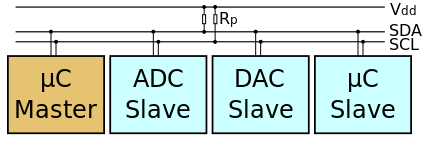
\includegraphics[width=0.85\textwidth, keepaspectratio]{imatges/I2C.png}
 \caption{Esquema d'un bus I2C típic}{Esquema d'un bus I2C típic. Font: user:Cburnett (Own work made with Inkscape) [GFDL o CC-BY-SA-3.0], via la Wikimedia Commons}
 \label{fig:I2C}
\end{figure}

\section{Exemple d'I2C}
\label{sub:I2C_example}
Per aquest exemple farem servir el sensor de gestos, de llum i de proximitat {\bf APDS-9960} de Broadcom \cite{apds9960}. Es pot adquirir una placa de prototipat a la web Sparkfun per poder provar-lo ràpidament. La placa té un connector força estàndard amb els pins d'alimentació, massa, les dues línies del \gls{I2C} \gls{SCL} i \gls{SDA}, i un pin d'interrupció.

Per connectar aquesta \gls{PCB} a la nostra placa de prototipat, farem servir 4 cables i els connectarem seguint la Taula~\ref{tb:I2C}.

\begin{table}
\caption{Connexionat de la placa APDS-9960 i la placa de prototipat}
\label{tb:I2C}
\centering
\begin{tabular}{|c|c|}
\hline
{\bf SiliconLabs (Expansion header)}	 & {\bf APDS-9960 PCB Board}\\
\hline
15 & SCL\\
\hline
16 & SDA\\
\hline
19 & GND\\
\hline
20 & VDD\\
\hline
\end{tabular}

\end{table}

Amb això estem connectant directament els pins del microcontrolador que poden fer de màster \gls{I2C} als pins sensor que fa d'slave I2C. Les resistències de \gls{pull-up} que calen per tot bus I2C estan a la PCB d'sparkfun (veure a l'esquemàtic aquí les resistències R2 i R3).

Un cop tenim el Hardware preparat, cal posar-se amb el Firmware. Per fer servir el controlador Màster del nostre microcontrolador podem fer sevir les llibreries de SiliconLabs emlib. \href{https://github.com/mariusmm/cursembedded/tree/master/Simplicity/I2C_1}{Aquí està el projecte sencer} per EFM32.

El primer que cal fer és activar el rellotge per aquest perifèric i configurar els pins corresponents. En aquest cas, els pins 15 o 16 del connector corresponent als pins PD7 i PD6 respectivament, que són la {\em localization \#1} del I2C d'aquest microcontrolador (Llistat~\ref{i2cpins}).
\index{CMU{\_}ClockEnable()}\index{GPIO{\_}PinModeSet()}
\begin{lstlisting}[frame=single,style=customc, label=i2cpins, caption={Initialització dels pins per l'I2C}]
CMU_ClockEnable(cmuClock_I2C0, true);
GPIO_PinModeSet(gpioPortD, 7, gpioModeWiredAnd, 1);
GPIO_PinModeSet(gpioPortD, 6, gpioModeWiredAnd, 1);

I2C0->ROUTE = I2C_ROUTE_SDAPEN | I2C_ROUTE_SCLPEN |
        I2C_ROUTE_LOCATION_LOC1;
\end{lstlisting}

A continuació cal configurar el perifèric màster, podem deixar-ho tot amb les opcions per defecte (Llistat~\ref{i2cconfig}).

\index{I2C{\_}Init()}
\begin{lstlisting}[frame=single,style=customc,label=i2cconfig, caption={Inicialització del perifèric I2C}]
I2C_Init_TypeDef i2cInit = I2C_INIT_DEFAULT;
I2C_Init(I2C0, &i2cInit);
\end{lstlisting}

Un cop fet això, ja podem fer servir el controlador I2C per accedir als dispositius que hi hagin al bus.

Per comoditat, s'acostuma a munta una funció per llegir registres i una funció per escriure'n. Veiem la funció {\bf I2C\_ReadRegister()}\index{I2C{\_}ReadRegister()} (Llistat~\ref{I2CReadRegister}).
\index{I2C{\_}TransferInit()}\index{I2C{\_}Transfer()}
\begin{lstlisting}[style=customc,caption=Funció {\bf I2C\_ReadRegister},label=I2CReadRegister]
static bool I2C_ReadRegister(uint8_t reg, uint8_t *val) {
  I2C_TransferReturn_TypeDef I2C_Status;
  I2C_TransferSeq_TypeDef seq;
  uint8_t data[2];

  seq.addr = DEVICE_ADDR;
  seq.flags = I2C_FLAG_WRITE_READ;
  seq.buf[0].data = &reg;
  seq.buf[0].len = 1;
  seq.buf[1].data = data;
  seq.buf[1].len = 1;

  I2C_Status = I2C_TransferInit(I2C0, &seq);

  while (I2C_Status == i2cTransferInProgress) {
    I2C_Status = I2C_Transfer(I2C0);
  }
  if (I2C_Status != i2cTransferDone) {
    return false;
  }
  *val = data[0];
  return true;
}
\end{lstlisting}

El primer que fem és definir les variables que ens caldran. La variable més estranya que veiem aquí és la variable {\bf seq} de tipus {\bf I2C\_TransferSeq\_TypeDef}. En aquesta estructura és on es guarda tota la informació necessària per engegar una transacció per part del controlador dins el microcontrolador. Per tant, a l'estructura cal posar-hi l'adreça \gls{I2C} del dispositiu, quina mena de transacció es vol fer (lectura, escriptura, etc.), en aquest cas {\bf I2C\_FLAG\_WRITE\_READ}, que vol dir que volem llegir d'un registre; també cal omplir una {\em array} d'estructures ({\bf buf[]}) on es guarda les dades a enviar o a rebre. En aquest cas, com que només volem llegir un registre (un sol byte) al {\bf buf[0]} només hi posem l'adreça del registre a llegir i la longitud a 1 i a {\bf buf[1]} li posem un {\em buffer} per emmagatzemar el valor llegit i de longitud 1 sol byte per llegir.

Un cop omplerta aquesta estructura s'engega la transacció amb la crida {\bf I2C\_TransferInit()}\index{I2C{\_}TransferInit()}, que retorna un {\bf I2C\_Status}. Després, tal com ens demana la biblioteca EMLIB, cal anar cridant la funció {\bf I2C\_Transfer()}\index{I2C{\_}Transfer()} mentre la variable {\bf I2C\_Status} valgui {\bf i2cTransferInProgress}. Això indica que la transferència pel bus s'ha acabat i cal veure com ha anat l'operació. Si tot ha anat bé la variable {\bf I2C\_Status} valdrà {\bf i2cTransferDone}. Així, el que tenim és una funció que li passem l'adreça del registre que volem llegir i ens retorna el valor que ens retorna el dispositiu.

Ara tornem al nostre sensor de gestos. Quasi tots els dispositius I2C tenen un registre de tipus identificació, que ens permet validar que la comunicació es fa realment amb ell. En el cas del APDS-9960 té un registre anomenat ‘ID' a l'adreça 0x92 i que el valor que retorna al llegir-lo és 0xAB (pàgina 25 del {\em Datasheet} \cite{apds9960}). Ara toca, doncs, muntar una funció que comprovi que s'està correctament a aquest dispositiu:

\index{testI2C()}\index{I2C{\_}ReadRegister()}
\begin{lstlisting}[style=customc,caption=Funció {\bf testI2C()},label=testI2C]
void testI2C(void) {
  uint8_t ret_value;

  I2C_ReadRegister(0x92, &ret_value);

  if (ret_value == 0xAB) {
    printf("Detected!\r\n");
  } else {
    printf("Something went wrong\r\n");
  }
}
\end{lstlisting}

Ara només cal ajuntar-ho tot en el nostre main i ja podem comprovar que tenim la PCB ben connectada i funcionant. Farem servir aquest bus i el mateix dispositiu a l'exemple tractat a \fullref{ch:aplicaciosenzilla}.


\chapter{SPI}
\label{sub:SPI}
El bus \gls{SPI} és un altre dels busos més populars usats en sistemes encastats. Aquest sistema de comunicació no és un bus pròpiament dit, donat que ens permet connectar un {\em Master} amb un {\em Slave} i només de forma indirecta connectar més {\em Slaves}.
Aquest bus es basa en dues línies per enviar o rebre dades, batejades \gls{MOSI} i \gls{MISO} segons la dada vagi del {\em Master} cap a l'{\em Slave} o a l'inrevés. Com és un bus síncron, hi ha una tercera línia que porta el rellotge (\gls{SCLK}) i que el genera el {\em master}. Per últim, hi ha una quarta línia de control, normalment anomenada \gls{SS} que indica a un {\em slave} concret que la transmissió és per ell. Controlant correctament un conjunt d'aquestes línies \gls{SS} és possible tenir més dispositius {\em slaves} al connectats al bus (Figura~\ref{fig:SPI}). Aquesta línia pot no usar-se, i llavors es parla d'un SPI de 3 fils enlloc d'un SPI de 4 fils.


\begin{figure}
 \centering
 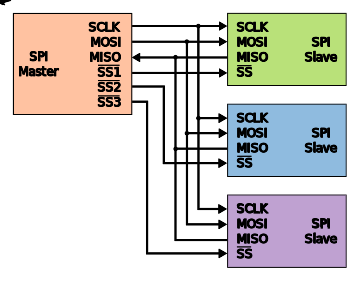
\includegraphics[width=0.85\textwidth, keepaspectratio]{imatges/SPI_three_slaves.png}
 \caption{Bus SPI típic}{Bus SPI típic. Per en:User:Cburnett [GFDL (http://www.gnu.org/copyleft/fdl.html) o CC-BY-SA-3.0 (http://creativecommons.org/licenses/by-sa/3.0/)], de la Wikimedia Commons}
 \label{fig:SPI}
\end{figure}




Aquest bus acostuma a poder treballar a força més velocitat que el bus \gls{I2C}, i és habitual configurar-lo per freqüències de rellotge d'uns pocs MHz (és habitual treballar amb freqüències d'1, 10 o fins i tot 24 MHz). En tot cas, cal consultar sempre les especificacions dels dispositius {\em slave} per saber la velocitat màxima de treball.

Precisament per aquesta característica, que fa que es puguin enviar moltes més dades per segon, els dispositius que incorporen un bus SPI acostumen a ser sensor i dispositius que generen un gran volum de dades de forma continua, com ara: \glspl{ADC}, memòries RAM i \gls{FLASH}, LCDs, targetes SD,  alguns sensors concrets, etc.

Com que aquest bus no està pensat per tenir més d'un {\em slave} connectat simultàniament, no incorpora el concepte d'adreça de dispositiu. A diferència del \gls{I2C}, que el propi bus especifica com és el protocol per accedir a un registre, en el SPI aquesta definició és pròpia de cada fabricant. Tot i això, habitualment el primer camp de la transmissió és l'adreça del registre a accedir o la comanda a executar.

En alguns microcontroladors el control d'aquest bus el fa el perifèric USART (veure \fullref{sub:UART}) configurat pertinentment, com és el cas de les famílies de microcontroladors de Silicon Labs \cite[207]{EFM32GRM}, i d'altres famílies incorporen perifèrics dedicats en exclusiva a aquest bus, com els de ST \cite[873]{STM32F4RM}.

\chapter{DMA}
\label{sub:DMA}
El \gls{DMA} és un dispositiu present a la majoria de microprocessadors. Aquest dispositiu s'encarrega de fer transferències de dades entre dispositius o memòria sense que la CPU intervingui.

Per què es fa servir? Doncs perquè sovint cal transferir quantitats importants de dades entre dues parts de la memòria, o anar transferint dades d'un dispositiu cap a un {\em buffer} a la memòria i no cal que la CPU estigui entretinguda fent això quan podria fer alguna cosa més interessant o en un mode de baix consum (veure~\fullref{ch:low-power}).

Els DMA acostumen a tenir diferents canals que poden fer transferències per separat i en paral·lel, de manera que podem tenir un canal preparat per moure regions de memòria, un altre per enviar dades cap a un DAC, un tercer transferint les dades rebudes per la UART, etc. Aquest diferents canals acostumen a estar prioritzats, de manera que l'àrbitre del bus pot decidir quin canal ha de poder accedir abans que un altre.

Normalment el dispositiu DMA es configura mitjançant descriptors, que són unes estructures on es guarda el tipus de transferència, l'adreça d'origen, l'adreça de destí, etc. Un cop s'engega la transferència, el DMA anirà movent les dades d'una adreça a l'altra segons s'hagi configurat. A la majoria de DMAs moderns, a més, es pot configurar el DMA de manera que copiï una dada d'un determinada adreça (que correspon a un registre de dades d'un perifèric) cada cop que el perifèric llença una notificació, de manera que el DMA fa una còpia d'una dada cada cop que el dispositiu en genera una. Tot això es veurà millor amb dos exemples.

\section{Exemple}
\label{sub:DMA_example}
Posar un exemple de \gls{DMA} sovint és complicat, ja que involucra força perifèrics diferents i configuracions, així que intentarem fer algun de simple per començar. Per aquest \href{https://github.com/mariusmm/cursembedded/tree/master/Simplicity/DMA_1}{primer exemple} hem optat per fer una transferència entre dues regions de memòria amb el DMA. Per això, tindrem un buffer d'origen i un de destí, en aquest cas de 256 elements de 32 bits cadascun (uint32\_t src\_buffer[BUFFER\_SIZE]).

El primer que es fa és inicialitzar el DMA amb les funcions d'emlib corresponents.
\index{DMA{\_}Init()}
\begin{lstlisting}[caption={Inicialització del DMA},style=customc]
dma_init.hprot = 0;
dma_init.controlBlock = dmaControlBlock;
DMA_Init(&dma_init);
\end{lstlisting}

La variable {\bf dmaControlBlock} és un {\em array} on es guarden els descriptors de cada un dels canals disponibles del DMA (Llistat~\ref{dmaControlBlock}).
\begin{lstlisting}[style=customc, caption={Definició de la variable {\bf dmaControlBlock}}, label=dmaControlBlock]
DMA_DESCRIPTOR_TypeDef dmaControlBlock[DMACTRL_CH_CNT * 2] SL_ATTRIBUTE_ALIGN(DMACTRL_ALIGNMENT);
\end{lstlisting}

A continuació configurem un canal del DMA (Llistat~\ref{DMAchannelconfig}) i li assignem una funció de \gls{callback} perquè ens notifiqui quan ha acabat la transferència (Llistat~\ref{DMAComplete}):
\index{DMA{\_}CfgChannel()}
\begin{lstlisting}[style=customc, caption={Configuració del canal DMA}, label=DMAchannelconfig]
dma_cb.cbFunc = DmaComplete;
dma_cb.userPtr = NULL;

dma_chn.enableInt = true;
dma_chn.highPri = false;
dma_chn.select = 0; /* set to 0 because is a memory-to-memory transfer */
dma_chn.cb = &dma_cb;
DMA_CfgChannel(0, &dma_chn);
\end{lstlisting}

\begin{lstlisting}[style=customc,caption={Callback del DMA {\bf DmaComplete()}\index{DmaComplete()}},label=DMAComplete]
void DmaComplete(unsigned int channel, bool primary, void *user) {
  dma_end = true;
}
\end{lstlisting}
També s'activen les interrupcions (necessàries per tenir \glspl{callback}) i es selecciona com serà la transferència (en aquest cas un 0 per indicar que serà de memòria a memòria).

Per últim es configura el descriptor de la transferència (Llistat~\ref{paramDMA}).
\index{DMA{\_}CfgDescr()}
\begin{lstlisting}[style=customc, caption={Paràmetres de configuració del DMA}, label=paramDMA]
dma_descr.arbRate = dmaArbitrate1;
dma_descr.dstInc = dmaDataInc4;
dma_descr.hprot = 0;
dma_descr.size = dmaDataSize4;
dma_descr.srcInc = dmaDataInc4;
DMA_CfgDescr(0, true, &dma_descr);
\end{lstlisting}

En aquest cas es tria com ha de manegar les adreces (tant a la font com al destí) i quants bytes es transfereixen a cada accés. Com que estem movent un {\em array} de 32 bits de paraula, triem incrementar de 4 en 4 l'adreça i moure 4 bytes a cada accés.

Per últim activem la transferència \gls{DMA} com es veu al Llistat~\ref{activateDMA}.
\index{DMA{\_}ActivateAuto()}
\begin{lstlisting}[style=customc, caption={Activació de la transferència DMA}, label=activateDMA]
DMA_ActivateAuto(0, true, dst_buffer, src_buffer, BUFFER_SIZE - 1);
\end{lstlisting}

Aquí la única particularitat és que cal especificar-li el nombre d'accessos a fer per completar la transferència, però restant-li un\footnote{Això és una particularitat de la biblioteca EMLIB de {\em Silicon Labs}} i altres biblioteques poden necessitar paràmetres lleugerament diferents.

A l'exemple es fa servir una variable global (volatile!) de nom {\bf dma\_end} que la \gls{callback} posa a {\em true} per notificar que la transferència s'ha acabat a la funció {\bf main()}. Quan això passa, es comprova que els dos {\em buffers} són iguals (Llistat~\ref{Check_buffers}) i es presenta per la consola.

\index{check\_buffers\_copy()}
\begin{lstlisting}[style=customc, caption={Comparació dels dos buffers de l'exemple DMA}, label=Check_buffers]
bool check_buffers_copy() {
  int i;

  for (i=0; i<BUFFER_SIZE; i++) {
    if (dst_buffer[i] != src_buffer[i]) {
      return false;
    }
  }
  return true;
}
\end{lstlisting}


\section{Un exemple amb DMA més complicat}
\label{sec:DMA_example_2}

Una altra aplicació del \gls{DMA} és transferir dades cap o des de un perifèric cap a memòria sense que el processador ho hagi de fer. Un exemple és fer servir el DMA per rebre o transferir dades cap al port sèrie. Així, enlloc d'anar llençant una \gls{IRQ} cada cop que el microcontrolador pot enviar la següent dada, es pot configurar el DMA per a que ho faci ell mateix de forma automàtica Anem a veure com es fa això modificant el \href{https://sistemesencastats.wordpress.com/2018/03/08/serie-i-usb-cp2102/}{segon exemple sobre la UART} (comentat a la \fullref{sec:UART_example_2}).

Així, el que farem en aquest exemple és deixar el \gls{buffer circular} i el mateix mecanisme per rebre dades de la {\bf USART (RX)} però canviarem la manera en que enviem les dades (TX). L'exemple és \href{https://github.com/mariusmm/cursembedded/tree/master/Simplicity/UART_DMA}{aquí}.

El que farem és preparar el DMA per a que transfereixi dades des d'un {\em buffer} a la memòria cap al registre d'enviament de la USART (registre {\bf TXDATA} de la USART1). En aquest cas, cal configurar-lo que no incrementi l'adreça de destí, que incrementi la font byte a byte i que transfereixi bytes (els caràcters d'una UART són bytes). També cal especificar quin dispositiu fa de {\em trigger}, és a dir, quin dispositiu notifica que té una dada disponible per ser transferida (paràmetre dma\_chn.select = DMAREQ\_USART1\_TXBL). En aquest exemple no ens cal saber quan el \gls{DMA} ha acabat la transferència, així que no registrem cal \gls{callback} ni activem les interrupcions del DMA. Tot això ho hem encapsulat a la funció {\bf my\_DMA\_Init()}\index{my{\_}DMA{\_}Init()} (Llistat~\ref{DMAinit_2}).

\index{my{\_}DMA{\_}Init()}
\begin{lstlisting}[style=customc,caption={Diferències a la inicialització del DMA}, label=DMAinit_2]
void my_DMA_Init(void) {
  ...
  dma_chn.select = DMAREQ_USART1_TXBL;
  ...
  dma_descr.dstInc = dmaDataIncNone;
  dma_descr.size = dmaDataSize1;
  dma_descr.srcInc = dmaDataInc1;
  ...
}
\end{lstlisting}

Ens cal també una funció que engegui la transferència del DMA cap a la UART. Li hem dit {\bf sendUARTbyDMA()}\index{sendUARTbyDMA()} i rep com a paràmetres el {\em buffer} a enviar i la seva longitud (en bytes). Aquesta funció tan sols espera que el DMA no estigui ocupat i tot seguit engega la transferència (veure Llistat~\ref{lst:sendUARTbyDMA}).

\index{sendUARTbyDMA()}\index{DMA{\_}ChannelEnabled()}\index{DMA{\_}ActivateBasic()}
\begin{lstlisting}[style=customc, caption={Funció sendUARTbyDMA()}, label=lst:sendUARTbyDMA]
void sendUARTbyDMA(void *buffer, int size) {
  /* wait for other DMA transfer to complete */
  while (DMA_ChannelEnabled(DMA_USART_TX_CHANNEL));

  /* Activate DMA */
  DMA_ActivateBasic(DMA_USART_TX_CHANNEL, true, false, (void *) &(USART1->TXDATA), buffer, size - 1);
}
\end{lstlisting}

La resta del codi és prou auto-explicatiu (o ho hauria de ser!): no s'activa la \gls{IRQ} de TX de la USART i hem tret la \gls{ISR} corresponent. Tampoc es crea un \gls{buffer circular} per enviar per la UART.

Dins el bucle infinit del {\bf main()}\index{main()} s'espera a rebre un caràcter, es munta una cadena relativament llarga (17 bytes) amb el caràcter rebut i per acabar s'envia usant la nova funció.
\index{AvailableData()}\index{PopData()}\index{sendUARTbyDMA()}\index{sprintf()}
\begin{lstlisting}[style=customc, caption={funció {\bf main()} de l'exemple}]
void main() {
  ...
  while (1) {
    if (AvailableData(&RX_SerialBuffer) != 0) {
      character = PopData(&RX_SerialBuffer);
      sprintf(TXbuffer, "Send by DMA (%c)\r\n", character);
      sendUARTbyDMA(TXbuffer, strlen(TXbuffer));
    }
  }
  ...
}
\end{lstlisting}

Per veure com connectar i fer servir el port sèrie per comunicar-se amb un ordinador, mireu el \fullref{sub:UART}.

\chapter{FLASH}
\label{ch:FLASH}
La memòria \gls{FLASH} que actua com a \gls{ROM} pel nostre microcontrolador també es pot fer servir per emmagatzemar dades d'usuari i ser escrita i llegida per codi de programa. Com que aquesta mena de memòria és no volàtil, les dades que hi guardem romandran entre reinici o pèrdues d'alimentació.

Cal tenir en compte que les memòries FLASH tenen certes particularitats que les fan diferents a d'altre tipus de memòries:
\begin{itemize}
 \item Número finit de cicles d'escriptura i lectura: les memòries FLASH tenen un límit de vegades que es poden esborrar i escriure. Aquest nombre pot estar entre 10.000 i 100.000 cicles, cosa que les pot fer poc adequades per emmagatzemar dades que variïn molt sovint.
 \item Paginació: les memòries FLASH estan organitzades en pàgines que cal esborrar sencera per escriure una dada.
 \item No es pot llegir mentre s'escriu la memòria FLASH del microcontrolador, per tant caldrà tenir una cura especial en que no hi hagi cap lectura ni execució de codi (compte amb les \glspl{ISR}) mentre s'està escrivint dades a la FLASH.
\end{itemize}

En el cas dels microcontroladors de Silicon Labs, el nombre màxim d'escriptures a la \gls{FLASH} és de 20.000 cicles, un cop passada aquesta xifra la FLASH pot començar a donar problemes \cite[28]{EFM32ZG108DS} (en els microcontroladors d'ST, el nombre de cicles garantits és de 10.000 \cite[110]{STM32F4DS}). Això fa que, per exemple, si volem emmagatzemar les dades d'un sensor que es llegeixen cada 10 segons a la FLASH, estaríem superant les 20.000 escriptures al cap de 55 dies de funcionament. Caldrà buscar mètodes alternatius d'emmagatzemar les dades per tal de no fer malbé la \gls{FLASH} tant aviat.

\section{Un exemple senzill}
A continuació veurem un exemple senzill on guardarem un conjunt de dades que han de ser persistents entre reinicis o pèrdues d'alimentació del nostre dispositiu. L'exemple està al repositori amb el nom de \href{https://github.com/mariusmm/cursembedded/tree/master/Simplicity/FLASH_1}{FLASH\_1}.

Primer es defineix una estructura en C per agrupar les dades que es volen emmagatzemar a la \gls{FLASH} tal com es veu al Llistat~\ref{structFLASH}. Tots els camps d'aquesta estructura seran les dades persistents que guardarem a la FLASH i que es podran llegir de nou a cada reinici.
\begin{lstlisting}[style=customc,caption={Estructura per guardar-se a la FLASH},label=structFLASH]
typedef struct {
  uint32_t field1;
  uint8_t  field2;
  uint32_t field3;
  bool	   field4;
} persistent_data_t;
\end{lstlisting}

Tot seguit es defineixen dues funcions per llegir i escriure a la \gls{FLASH} (Llistat~\ref{FLASH_functions}). Com es pot veure, cal cridar a funcions especials per escriure a la FLASH: la primera ({\bf MSC\_ErasePage()}\index{MSC\_ErasePage()}) esborra una pàgina de la FLASH i la segona ({\bf MSC\_WriteWord()}\index{MSC\_WriteWord()}) escriu a la FLASH les dades que se li passin. Aquesta funció d'escriptura necessita que la mida de les dades sigui divisible per 4 (en el cas de la nostra estructura, la seva mida es 16 bytes) \cite{FLASH_EFM32}\cite{EMLIB_MSC}.

\index{Flash\_Write()}\index{Flash\_Read()}\index{MSC\_ErasePage()}\index{MSC\_WriteWord()}
\begin{lstlisting}[style=customc,caption={Funcions per accedir a la FLASH},label=FLASH_functions]
void Flash_Write() {
  MSC_ErasePage(userDataPage);
  MSC_WriteWord(userDataPage, &my_persistent_data, sizeof(my_persistent_data));
  printf("Data stored in Flash\r\n");
}

void Flash_Read() {
  memcpy(&my_persistent_data, userDataPage, sizeof(my_persistent_data));
}
\end{lstlisting}

Com es pot veure al mateix codi (Llistat~\ref{FLASH_functions}), per llegir de la memòria \gls{FLASH} (funció {\bf Flash\_Read()}\index{Flash\_Read()}) només cal fer un accés a memòria normal i corrent, i en aquest cas el que es fa és copiar el contingut de la FLASH cap a la estructura amb les dades persistents amb un {\bf memcpy()}.

La resta de l'exemple és prou senzill: quan es prem el botó 0 de la placa d'avaluació s'escriu a la FLASH l'estructura i al pitjar el botó 1 es canvien els valors de dita estructura. D'aquesta manera, al iniciar la sessió de {\em debug} es pot observar com els valors que hi han guardat a la FLASH i que es copien a l'estructura són els valors que s'han guardat prèviament a l'anterior execució.

Per últim, cal fer notar que la macro {\bf USERDATA\_BASE} està definida pel fabricant i apunta a la zona de la FLASH reservada per l'usuari d'una pàgina (en aquest cas 512 bytes) de longitud.

\section{\em Bootloaders}
\label{sec:Bootloader}
Un cas especial per accedir a la \gls{FLASH} és el dels {\em bootloaders}. Un {\em bootloader} és un petit codi que s'executa cada cop que s'inicia el microcontrolador i acostuma a poder gestionar la reprogramació del microcontrolador d'una forma més amigable que no pas usant el programador.

El més habitual en {\em bootloaders} per sistemes encastats és que puguin rebre una nova imatge de l'executable de l'aplicació a través d'un dels ports sèrie del sistema \footnote{També hi ha {\em bootloaders} que poden rebre la imatge per USB, via ràdio, per un port Ethernet, llegir-la d'una tarja SD, etc.}. Per realitzar aquest tasca, el {\em bootloader} ha de poder accedir i escriure a tota la memòria FLASH del microcontrolador \cite{AN0003}.

\chapter{Altres perifèrics}
\label{ch:otherperipherals}
Fins ara s'han introduït els perifèrics més habituals i que es poden trobar a als microcontroladors actuals. Tot i això, hi ha altres perifèrics més específics d'algun àmbit d'aplicació que no s'han presentat. En podem enumerar uns quants sense poder ser exhaustius:

\begin{itemize}
 \item Mòduls {\em crypto} que permeten operacions de tipus criptogràfic per realitzar càlculs de claus criptogràfiques. Sovint aquesta mena de mòduls suporten directament el xifratge o desxifratge en estàndards com AES, DES, triple-DES, etc. \cite[720]{STM32F4RM}\cite[772]{STM32F4RM}\cite[453]{EFM32TGRM}.
 \item \gls{DMA} avançats, que permeten fer transferències complexes, no tant sols d'un {\em buffer} d'una sola dimensió (com els {\em arrays}) si no de dues dimensions per moure imatges o matrius de 2 dimensions \cite[339]{STM32F4RM}.
 \item {\em Drivers} \gls{LCD} que poden controlar directament pantalles \cite[480]{STM32F4RM}\cite[490]{EFM32TGRM}. Segons el model i el fabricant aquest mòdul podrà controlar diferents tipus de pantalla (LCD o TFT), amb color o blanc i negre, diferents resolucions i profunditat de color, etc.
 \item Mòdul controlador de USB que permet connectar i controlar el microcontrolador al bus USB \cite[965]{STM32F4RM}\cite[1446]{EFM32GG11RM}.
 \item Mòdul Ethernet per poder connectar el nostre sistema encastat a una xarxa cablejada amb Ethernet. Aquests tipus de perifèrics necessiten un xip extern que es controla per un bus força estandarditzat anomenat \gls{MII} (o el més modern RMII) \cite[1121]{STM32F4RM}\cite[1729]{EFM32GG11RM} \cite{wiki:rmi}.
 \item Controlador \gls{SDIO} per accedir a dispositius SDIO, majoritàriament targetes de memòria SD \cite[1019]{STM32F4RM}\cite[1670]{EFM32GG11RM}.
 \item Controlador de bus \gls{CAN} que permet connectar el dispositiu al bus CAN \cite[1076]{STM32F4RM}\cite[1899]{EFM32GG11RM} \cite{wiki:can}.
\end{itemize}

Treballar amb aquests perifèrics, tot i que no ho veurem en aquest llibre, és força similar a la resta de perifèrics que hem vist: estan mapats a memòria i tenen un conjunt de registres que permet controlar el perifèric a través de llegir i escriure aquests registres. Els fabricants proporcionen biblioteques per facilitar-ne l'ús com amb la resta de perifèrics que hem vist.

Els perifèrics més complexos (per exemple USB o Ethernet) acostumen a portar associats una biblioteca proporcionada pel fabricant o per tercers per poder controlar el perifèric i simplificar-ne l'ús. Així, per exemple, és habitual fer servir la biblioteca LwIP per tenir funcionalitat de xarxa ({\em sockets}, TCP, UDP, IP, etc.) \cite{lwip}\cite{wiki:lwip} i que els fabricants proporcionin documentació o codi per enllaçar aquesta biblioteca amb el seu perifèric.

\chapter{Una aplicació completa}
\label{ch:aplicaciosenzilla}
Ja va sent hora de fer una aplicació completa (senzilla) per il·lustrar tot el que hem anat aprenent durant el curs.

Anem a veure una \href{https://github.com/mariusmm/cursembedded/tree/master/Simplicity/Barebone_App_1}{aplicació sencera} on ajuntarem unes quantes coses de les que hem vist fins ara. Farem una aplicació que segons la proximitat de la ma al sensor (o del sensor a una taula o un obstacle), faci pampallugues més ràpid o més lent el LED de la PCB. Farem servir el sensor de proximitat APDS-9960 connectat a la nostra placa de prototipat com ja vàrem fer a l'exemple d'I2C. Per tant, caldrà anar llegint cíclicament el sensor de proximitat i canviar el valor de \gls{PWM} del LED segons el valor llegit.

Com que aquest projecte fa servir diferents perifèrics del microcontrolador i les seves llibreries, cal organitzar el codi perquè tot sigui entenedor i amb un manteniment senzill. Així, tindrem un conjunt de mòduls (se li mòdul a una parella de fitxers .c i .h) per manegar les diferents funcionalitats, sensors i perifèrics. Per últim, tindrem el fitxer {\em main.c} on hi ha la funcionalitat principal de l'aplicació.

\section{Biblioteques}
Aquesta aplicació fa servir quatre biblioteques per organitzar el codi, anem a descriure-les amb detall.

\subsection{BSP}
Habitualment en aquest mòdul s'hi posen les configuracions i inicialitzacions de diferents perifèrics o dispositius comuns a tot el sistema.

En aquest cas es gestiona algun dels rellotges del sistema, el pin corresponent al LED i es configura la sortida de la consola pel {\bf printf}.

D'aquesta biblioteca es fa servir la funció {\bf setupSWOForPrint()}\index{setupSWOForPrint()} i la funció {\bf BSP\_Init()}\index{BSP{\_}Init()}. Aquesta segona funció tant sols crida la primera i inicialitza el LED de la placa (que no es fa servir).

\subsection{I2C\_Wrapper}

Hem escrit una biblioteca senzilla per accedir al bus \gls{I2C} fent servir la llibreria emlib. D'aquesta manera encapsulem tota la funcionalitat en dues funcions senzilles de fer servir per llegir o escriure un registre d'un dispositiu I2C ({\bf I2C\_WriteRegister}\index{I2C{\_}WriteRegister()} i {\bf I2C\_ReadRegister}\index{I2C{\_}ReadRegister()}) com ja es va fer a \fullref{sub:I2C_example}.

\index{I2C{\_}WriteRegister()}\index{I2C{\_}TransferInit()}\index{I2C{\_}Transfer()}
\begin{lstlisting}[style=customc, caption={Part de la funció {\bf I2C\_WriteRegister}}, label=I2CWriteRegister]
bool I2C_WriteRegister(uint8_t addr, uint8_t reg, uint8_t data) {
  ...
  I2C_Status = I2C_TransferInit(I2C0, &seq);

  while (I2C_Status == i2cTransferInProgress) {
    I2C_Status = I2C_Transfer(I2C0);
  }
  ...
}
\end{lstlisting}


\subsection{PWM}
És una biblioteca molt senzilla per controlar el canal PWM que correspon al LED de la nostra placa. Només suporta aquest canal i només proporciona una funció per controlar el PWM, amb un paràmetre amb el percentatge de \gls{duty cycle} del PWM (100\% equival al LED sempre encès i 0\% correspon al LED apagat).
La funció {\bf PWM\_Init()}\index{PWM{\_}Init()} configura el Timer1 perquè funcioni com a generador de \gls{PWM}, de manera molt similar a l'exemple \fullref{sub:PWM_example}.

L'altra funció de la biblioteca és {\bf PWM\_Set()}\index{PWM{\_}Set()}, que rep el percentatge del \gls{duty cycle} que ha d'estar a 1 i configura el Timer d'acord a aquest percentatge. Com que el Timer està configurat perquè compti fins a {\bf PWM\_FREQ} (que val 4096), cal passar del rang 0 -- 100 a 0 -- 4096. Un cop calculat el valor correcte, s'usa com a valor al comparador del {\em timer}.

\index{PWM{\_}Set()}\index{TIMER{\_}CompareBufSet()}
\begin{lstlisting}[style=customc,caption={Funció PWM\_Set()},label=PWMSet]
void PWM_Set(uint8_t percentage) {
  uint32_t pwm_value;
  ...
  /* convert to percentage (0 to 100) to range 0 - PWM_FREQ */
  pwm_value = percentage * PWM_FREQ / 100;

  TIMER_CompareBufSet(TIMER1, 1, pwm_value);
}
\end{lstlisting}


\subsection{APDS-9960}
Aquesta biblioteca controla el sensor APDS-9960 via el bus \gls{I2C}. Només gestiona la funcionalitat de sensor de proximitat (que pot fer força més coses).

\index{APDS{\_}9960{\_}InitProximity()}\index{I2C{\_}WriteRegister()}
\begin{lstlisting}[caption={Funció {\bf APDS\_9960\_InitProximity()}},style=customc,label=InitProximity]
void APDS_9960_InitProximity() {
  // Enable Proximity detection
  // ENABLE <- 5 & 2 & 0 bits
  I2C_WriteRegister(DEVICE_ADDR, APDS_ENABLE_REG, 0x25);

  /* LED Strength to 100mA, Proximity Gain control to 8x */
  I2C_WriteRegister(DEVICE_ADDR, APDS_CTRL_1_REG, 0x0C);

  /* LED_BOOST 300% 0111_0001*/
  I2C_WriteRegister(DEVICE_ADDR, APDS_CTRL_2_REG, 0x71);
}
\end{lstlisting}

La funció {\bf APDS\_9960\_InitProximity()}\index{APDS{\_}9960{\_}InitProximity()} (Llistat~\ref{InitProximity}) inicialitza el sensor per a què funcioni com a sensor de proximitat. Cal consultar el Datasheet per veure els registres que s'escriuen i quins valors es posen \cite{apds9960}.

\index{APDS{\_}9960{\_}ReadProximity()}\index{I2C{\_}ReadRegister()}
\begin{lstlisting}[caption={Funció {\bf APDS\_9960\_ReadProximity()}},style=customc,label=ReadProximity]
bool APDS_9960_ReadProximity(uint8_t *p_data) {
  uint8_t status;
  bool ret = false;

  I2C_ReadRegister(DEVICE_ADDR, APDS_STATUS_REG, &status);

  if ((status & 0x02) != 0x00) {
    I2C_ReadRegister(DEVICE_ADDR, APDS_PDATA_REG, p_data);
    ret = true;
  }

  return ret;
}
\end{lstlisting}

La funció {\bf APDS\_9960\_ReadProximity()}\index{APDS{\_}9960{\_}ReadProximity()} (Llistat~\ref{ReadProximity}) llegeix el registre d'estatus i si hi ha una dada disponible la llegeix, la retorna a travès del paràmetre per referència i el retorn de la funció valdrà {\bf True}; si no hi ha una dada disponible retorna {\bf False}.

La biblioteca es basa en {\em polling} per saber si la dada a llegir és bona, comprovant el registre {\bf status} i retornant fals i no s'ha pogut llegir. Es podria millorar la biblioteca fent que el sensor llenci una interrupció cada cop que tingui una dada nova (es veurà més endavant a \fullref{sec:full_app_irq}).

\section{Funció principal}
La funció principal de l'aplicació està en el propi {\bf main()}\index{main()} i consta bàsicament d'un bucle sense fi on es va llegint el valor de proximitat del sensor (si està disponible) i s'ajusta el \gls{duty cycle} del \gls{PWM} segons aquest valor, de manera que el LED pampalluguegi més sovint quan més a prop estigui l'obstacle.

\index{APDS{\_}9960{\_}ReadProximity()}\index{PWM{\_}Set()}
\begin{lstlisting}[caption={Funció principal},style=customc,label=ProximityExample]
while(pdTrue) {
  ret = APDS_9960_ReadProximity(&p_data);

  if (ret == true) {
    printf("Proximity: %d\r\n", p_data);

    /* Convert from range 0 - 256 to 0 - 100 */
    PWM_Set((p_data * 100) / 256);
  }
}
\end{lstlisting}

Com que hem escrit la funció {\bf APDS\_9960\_ReadProximity()}\index{APDS{\_}9960{\_}ReadProximity()} de manera que retorni true o false segons si s'ha pogut llegir o no una dada, el codi ens queda molt senzill i llegible. Si s'ha pogut llegir, es treu per la consola de {\em debug} la dada i es converteix al rang adequat el valor llegit.

\begin{remark}
 Fixem-nos que la conversió de rang es fa forçant primer la multiplicació per 100 abans de la divisió per 256 per tal de no perdre precisió en la conversió. Com que treballem amb nombres enters, la divisió és entera i si ho féssim a l'inrevés obtindríem sempre valors 0, ja que <valor de 8 bits>/256 sempre dona 0 en una divisió entera i després encara que ho multipliquéssim per 100 seguiria donant 0..
\end{remark}


\section{Afegint-hi interrupcions}
\label{sec:full_app_irq}
En els exemples que hem vist fins ara, tant de perifèrics integrats com de dispositius externs la comunicació es feia via {\em pollin}, això és, preguntant tota l'estona si el dispositiu o perifèric té alguna dada disponible. L'altre manera de comunicar-se és mitjançant interrupcions, fent que el dispositiu o perifèric llenci una \gls{IRQ} cada cop que té una dada disponible.

Per això, ens calen almenys, fer els següents canvis al nostre sistema:
\begin{itemize}
 \item Connectar el pin d'\gls{IRQ} del sensor a la nostra placa de desenvolupament
 \item Configurar el sensor {\bf APDS-9960}, de manera que generi un senyal d'IRQ cada cop que tingui una nova dada disponible
 \item Habilitar les interrupcions al nostre microcontrolador perquè cridi la \gls{ISR} corresponent.
\end{itemize}

\subsection{Connexió del pin INT}
Per aconseguir connectar el pin INT del sensor {\bf APDS-9960} només cal fer servir un cinquè cable Dupont entre la placa de prototipat del sensor i la nostra placa de desenvolupament. Si mirem el manual de la placa de Silicon Labs, veurem que el pin PB12 es pot fer servir com a un GPIO normal i que generi una interrupció cada cop que tinguem un flanc.

Segons el {\em datasheet} \cite[3]{apds9960} del APDS-9960 el pin d'interrupció és de tipus \gls{open drain}. Això vol dir que aquest pin només pot forçar un valor '0' i li cal que el valor '1' estigui forçat per un \gls{pull-up}. En el cas de la placa que tenim, ja incorpora aquesta resistència de \gls{pull-up} Per tant, el pin de GPIO del microcontrolador no cal configurar-lo com entrada amb \gls{pull-up}.
\index{GPIO{\_}PinModeSet()}
\begin{lstlisting}[style=customc]
GPIO_PinModeSet(gpioPortB, 12, gpioModeInput, 1); /* IRQ from APDS_9960 */
\end{lstlisting}

Si la PCB no tingues la resistència de \gls{pull-up}, caldria configurar el pin com a \gls{pull-up} ja que si no ens trobaríem que sempre estaria a '0', ja que cap dels dos dispositius el posaria a '1'.

\subsection{Configurar el dispositiu APDS{\-}9960}
Ara cal que el sensor generi un senyal d'\gls{IRQ} cada cop que tingui una nova dada disponible.
% Veiem al {\em datasheet}\cite[p.20 i 21]{apds9960} que cal activar les interrupcions per proximitat (bit PIEN de l'Status Register) i posar uns valors adients als registres de {\em threshold} (adreces 0x88 i 0x89). Segons ens diu el {\em datasheet}, si el registre {\bf PDATA} està dins del nivell que marquen aquests dos registres es generarà una interrupció. Per últim, cal configurar el valor del camp {\bf PPERS} del registre {\bf Persistence} per
Veiem al {\em datasheet} \cite[11 i 20]{apds9960} que cal activar les interrupcions per proximitat (bit {\bf PIEN} del registre {\bf Status}) i si configurem el valor del camp {\bf PPERS} del registre {\bf Persistence} al valor 0 generarà una interrupció cada cop que hi hagi una dada nova.

\index{APDS{\_}9960{\_}InitProximity{\_}IRQ()}\index{I2C{\_}WriteRegister()}
\begin{lstlisting}[caption={Nova funció d'initialització del APDS{\_}9960},style=customc,label=APDS960InitProximityIRQ]
void APDS_9960_InitProximity_IRQ() {
  //Enable Proximity detection
  // ENABLE <- 5 & 2 & 0 bits
  I2C_WriteRegister(DEVICE_ADDR, APDS_ENABLE_REG, 0x25);

  /* LED Strength to 100mA, Proximity Gain control to 8x */
  I2C_WriteRegister(DEVICE_ADDR, APDS_CTRL_1_REG, 0x0C);

  /* LED_BOOST 300% 0111_0001*/
  I2C_WriteRegister(DEVICE_ADDR, APDS_CTRL_2_REG, 0x71);

  /* Generate IRQ every data valid */
  I2C_WriteRegister(DEVICE_ADDR, APDS_PERSISTENCE_REG, 0);
}
\end{lstlisting}

Amb aquesta configuració segons el {\em datasheet} el sensor posarà una interrupció cada cop que hi hagi una dada nova disponible de proximitat.

\subsection{Habilitar la interrupció corresponent}
L'últim pas és habilitar la interrupció corresponent al pin d'entrada que hem triat. És una operació molt similar al que ja s'ha vist a l'apartat dels GPIOs (\fullref{sub:GPIO_2}).

\index{GPIO{\_}IntConfig()}\index{NVIC{\_}EnableIRQ()}
\begin{lstlisting}[caption={Habilitar l'interrupció del pin corresponent},style=customc,label=APDS960EnableIRQ]
GPIO_IntConfig(gpioPortD, 8, false, true, true);
NVIC_EnableIRQ(GPIO_EVEN_IRQn);
\end{lstlisting}

Un cop tenim tot preparat, cal també modificar la nostra funció principal perquè no faci {\em polling}, que és el que volem evitar. Com que ara tenim una {\em ISR} que s'executarà cada cop que que hi hagi una dada nova al sensor, tenim vàries opcions, en destaquem dues:
\begin{itemize}
 \item Fer la lectura del registre del sensor des de la pròpia \gls{ISR}
 \item Activar un {\em flag} que ens indiqui que podem fer la lectura des de la funció principal.
\end{itemize}

Com ja s'ha comenta anteriorment (\fullref{ch:IRQ}) posar gaire codi dins una \gls{ISR} no és aconsellable, així que per aquest exemple farem servir la segona opció proposada. Per tant, afegirem una variable de tipus {\em bool} al projecte que farem servir com a {\em flag}. Aquest {\em flag} el posarem a {\bf true} dins la \gls{ISR} i la funció principal l'esborrarà cada cop que el faci servir (Llistats~\ref{APDS960ISRFlag} i \ref{APDS960Readmain}).

\index{GPIO{\_}EVEN{\_}IRQHandler()}\index{GPIO{\_}IntGet()}\index{GPIO{\_}IntClear()}
\begin{lstlisting}[caption={\gls{ISR} amb el {\em flag}},style=customc,label=APDS960ISRFlag]
void GPIO_EVEN_IRQHandler(void) {
  /* clear flags */
  aux = GPIO_IntGet();
  GPIO_IntClear(aux);

  signal = true;
}
\end{lstlisting}
\index{main()}\index{APDS{\_}9960{\_}ReadProximity()}
\begin{lstlisting}[caption={Funció principal amb suport d'interrupcions},style=customc,label=APDS960Readmain]
main() {
  ...
  while(signal == false);
  signal = false;

  ret = APDS_9960_ReadProximity(&p_data);
  ...
}
\end{lstlisting}

El que veiem a la funció {\bf main()}\index{main()} és que el microcontrolador estarà la major part del temps esperant a que el {\em flag} es posi a {\em true} per tal de continuar i poder fer l'operació de lectura del sensor i canviar el \gls{duty cycle} del \gls{PWM} del \gls{LED}. Tota aquesta estona que el microcontrolador està esperant-se sense poder fer res, es podrà aprofitar per posar-lo en algun mode de baix consum tal com veurem al \fullref{ch:low-power}.
